\documentclass[12 pt]{article}
\usepackage{graphicx}
% \usepackage{epstopdf}			% convert eps file to pdf
% \graphicspath{{/home/aliu/Documents/Latex/DFT DMFT userguide/DFT DMFT userguide versions/}}
\usepackage{amsmath} 			% math formatting
\usepackage{amssymb} 			% math symbols
\usepackage{amsthm}
\usepackage{enumitem}			% customize item labels
\usepackage{eulervm, bookman}		% fonts for math and symbols
\usepackage[round]{natbib} 		% bibliography styles
\usepackage{textcomp} 			% support text companion fonts
\usepackage{lipsum} 			% generate filler text
\usepackage[top=1in, bottom=0.5in, left=1in, right=1in, includefoot]{geometry} % set margins to 1 inch each side
\usepackage{fancyhdr} 			% change header
  \pagestyle{fancy} 			% change header to fancy style
  \fancyhead{} 				% empty the header
  \renewcommand{\headrulewidth}{0pt} 	% delete the header line
\usepackage{indentfirst} 		% first paragraph after section name is indented
\hfuzz=6pt 				% specifies the maximum amount of box overflow before a warning message is
					% being issued
\usepackage{filecontents} 		% add Bibliography to table of contents
\usepackage{tabularx}			% more table functions
\usepackage{chngcntr}			% set counter within or without part
\usepackage{appendix}			% appendix package to show Appendix title
%\usepackage{etoolbox}			% add hyperlinks in toc
\usepackage{pdflscape}			% pdflscape.sty produce landscape pages in a mainly portrait document
\usepackage{caption}			% caption centering
\usepackage{color}			% change the color of text

\usepackage{tikz}	
\usetikzlibrary{shapes}
\usetikzlibrary{arrows}
\usetikzlibrary{topaths}
\tikzstyle{DFT_DMFT} = [rectangle, minimum width=2.5cm, minimum height=1cm, text centered, draw=black, fill=red!30]
\tikzstyle{DFT} = [rectangle, rounded corners, minimum width=3cm, minimum height=1cm, text centered, draw=black, 
fill=blue!30]
\tikzstyle{DMFT} = [rectangle, rounded corners, minimum width=3cm, minimum height=1cm, text centered, draw=black, 
fill=orange!30]
\tikzstyle{impurity} = [ellipse, minimum width=3cm, minimum height=1cm, text centered, draw=black, fill=green!30]
\tikzstyle{arrow} = [line width=5pt, ->, >=latex]	
					% define tikz package to draw flow charts, line width, arrow tip

\title{
      {\Huge\textbf{User's Guide, DFTWIEN2k\_14.1+DMFT-Wien2K\_2012(2014)}}
      %\_\_\_\_\_\_\_\_\_\_\_\_\_\_\_\_\_\_\_\_\_\_\_\_\_\_\_\_\_\_\_\_\_\_\_\_\_\_\_\_\_\_\_\_\_\_\_\_\_\_\_\_\\
      } 				% adds title

\author{
      \large\textbf{Kristjan Haule$^\alpha$, Ang Liu$^\beta$, Peng Zhang$^\beta$ and Ronald Cohen$^\beta$}\\
      $\alpha$: Rutgers University, Piscataway, New Jersey\\
      $\beta$: Carnegie Institution of Washington, Washington, D.C.
      	} 				% adds author

\date{\today} 				% adds updated date
					% use .PNG image format whenever possible
					% save the image in same folder as . tex file

\linespread{2}				% set line spacing to double spacing

\makeatletter
\renewcommand\paragraph{%
    \@startsection{paragraph}{4}{0mm}%
    {-\baselineskip}%
    {.5\baselineskip}%
    {\normalfont\normalsize\bfseries}}
\makeatother				% Line break directly after paragraph title

\usepackage[pdfpagelabels, linktocpage, backref]{hyperref}	 
\hypersetup{	
  linkcolor=blue
  filecolor=magenta
  urlcolor=cyan
  bookmarks=true			% links in pdf, hyperref should be put bottom of preamble
}					% navigation friendly between contents and text

\begin{document}
   
  \begin{titlepage}
  \pagenumbering{Alph}			% change the invisible numbering of the title page
  \linespread{1.2}
  \maketitle

  \begin{figure}[h]
    \centering

    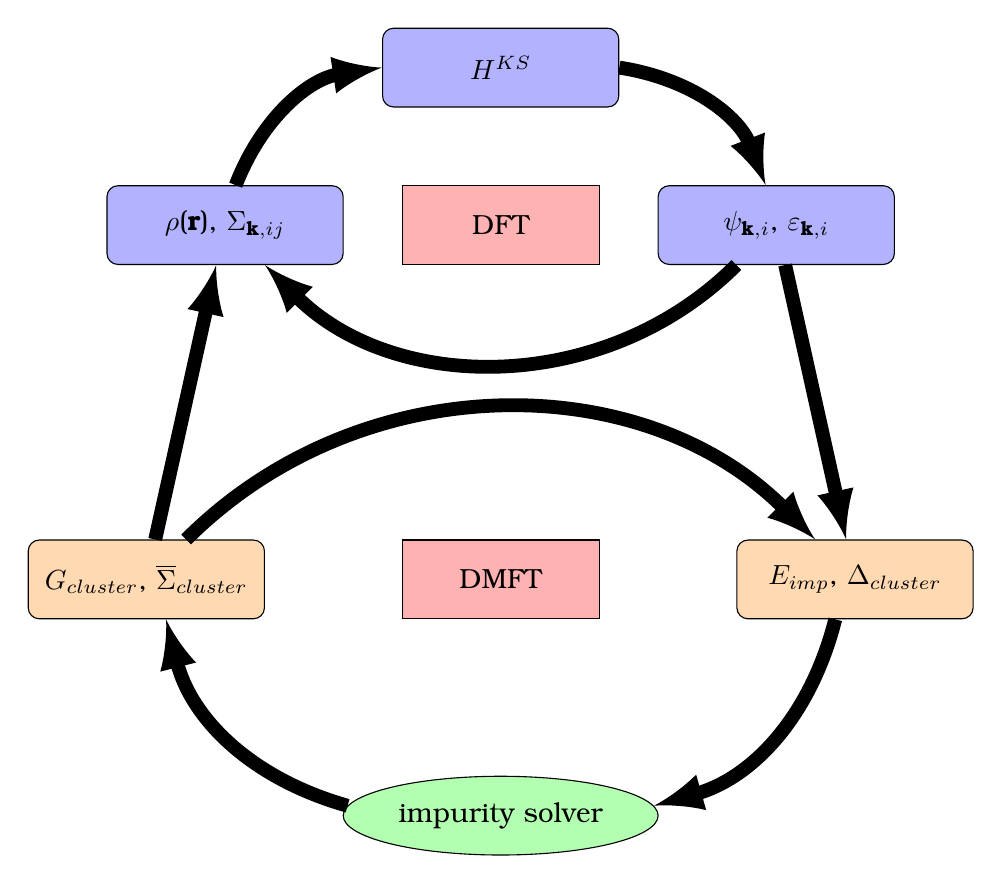
\begin{tikzpicture}[node distance=2cm]

    \node(DFT2)[DFT]{$H^{KS}$};
    \node(DFT)[DFT_DMFT, below of=DFT2]{DFT};
    \node(DFT1)[DFT, below of=DFT2, xshift=-3.5cm]{$\rho$(\textbf{r}), $\Sigma_{\textbf{k},ij}$}
	  edge[arrow, bend left=30](DFT2.west);
    \node(DFT3)[DFT, below of=DFT2, xshift=3.5cm]{$\psi_{\textbf{k},i}$, $\varepsilon_{\textbf{k},i}$}
	  edge[arrow, <-, bend right=30](DFT2.east)
	  edge[arrow, bend left=45](DFT1);

    \node(DMFT)[DFT_DMFT, below of=DFT, yshift=-2.5cm]{DMFT};
    \node(DMFT1)[DMFT, below of=DFT, yshift=-2.5cm, xshift=4.5cm]{$E_{imp}$, $\Delta_{cluster}$}
	  edge[arrow, <-](DFT3);
    \node(DMFT3)[DMFT, below of=DFT, yshift=-2.5cm, xshift=-4.5cm]{$G_{cluster}$, $\overline{\Sigma}_{cluster}$}
	  edge[arrow](DFT1)
	  edge[arrow, bend left=45](DMFT1);
    \node(DMFT2)[impurity, below of=DMFT, yshift=-1cm]{impurity solver}
	  edge[arrow, bend left=30](DMFT3)
	  edge[arrow, <-, bend right=30](DMFT1);

    \end{tikzpicture}

  \end{figure}

  \thispagestyle{empty} 		% suppress page number

  \end{titlepage}

  \makeatletter
  \renewcommand{\l@section}{\@dottedtocline{1}{1.5em}{2.6em}}
  \renewcommand{\l@subsection}{\@dottedtocline{2}{4.0em}{3.6em}}
  \renewcommand{\l@subsubsection}{\@dottedtocline{3}{7.4em}{4.5em}}
  \makeatother				% adjust spacing between the heading title and its number(the title margins)

  \newpage 				% add page before Contents
  \pagenumbering{roman} 		% set page numbering to small roman numerals
  \setcounter{page}{1} 			% reset page counter
  \renewcommand{\contentsname}{Table of Contents}
  \hypertarget{my toc}{}		% create a link back to Table of Contents
  \tableofcontents			% change Contents to Table of Contents
  \cleardoublepage
  \listoffigures			% list of figures
  \cleardoublepage
  \listoftables				% list of tables

  \newpage
  \pagenumbering{arabic} 		% change page numbering style from small roman to arabic
  \counterwithout{page}{part}		% reset page number
  \counterwithin{section}{part}

  \part{Introduction}

    One of the most challenging topics in condensed matter physics is the simulation and prediction of strongly 
correlated materials. The density functional theory plus dynamical mean-field theory (DFT+DMFT) method introduced in
 this userguide has been proven successful in fulfilling this target. The DFT+DMFT method is a combination of the 
traditional well-tested DFT method, in which the crystal problem is treated as the functional of electron density, 
and the DMFT method, where the local correlated physics is included in local self-energy. The DFT+DMFT method has 
been used in realistic simulations of strongly correlated materials, such as transition metals, lanthanides, 
actinides, as well as their compounds. We will give a detailed step-to-step introduction to the DFT+DMFT code in 
this userguide, from preparing the input files, checking whether the codes have arrived at converged and high-quality
 outputs, to how to extract realistic physical properties that can be compared with experiments.

This userguide is separated into four chapters: in the first chapter we give an introduction of the DFT+DMFT 
formalism; in the second chapter we present how to install the DFT+DMFT code; in the third chapter we present how to
 run the DFT+DMFT code, how to monitor the running, how to check if the outputs are converged, and how to improve the
 quality of your data; in the fourth chapter we use realistic examples to show the analysis of the DFT+DMFT output 
data, e.g. derivation of physical properties, such as density of states (DOS), momentum resolved spectra, optical 
conductivity, etc.

  The DFT+DMFT code has two parts: the DFT code and the DMFT code. In the DFT code, the inputs are atomic species and 
unit cell parameters. Its outputs are converged DFT Hamiltonian matrix at each k point and other parameters of the 
DFT Hamiltonian which are needed to construct local Green's function. The second part is the DMFT code. Inputs of 
DMFT are a choice of correlated orbitals and double counting, converged DFT Hamiltonian matrix and self-energy of 
previous iteration. After solving the DMFT equations with impurity solver, the local Green's function and new 
self-energy are fed back to the DFT iterations. There are three cycles in the DFT+DMFT codes, the DFT iterations, the
 DMFT iterations, and the DFT+DMFT charge self-consistent iterations. The final convergence is reached after the 
convergence of these three iterations.

  \begin{enumerate}
 
  \item The websites for downloading the source codes are shown below, 

  \begin{itemize}[leftmargin=0.5in]

    \item Where to download the \emph{WIEN2k} source code for DFT calculations (version WIEN2k\_14.1): 

  \url{http://www.wien2k.at/}

    \item Where to download the \emph{DMFT-Wien2K} source code for DMFT calculations (version 2012): 

  \url{http://hauleweb.rutgers.edu/downloads/}

  \end{itemize}

  \item The major references for WIEN2k and DFT+DMFT are listed below,

  \begin{itemize}[leftmargin=0.5in]

   \item The major reference for WIEN2k is shown here, 

  \citep{Haule2010}

   \item The major references for DFT+DMFT are shown here, 

  \citep{Blaha2001, Kotliar2004, Kotliar2006}

  \end{itemize}

  \end{enumerate}
  \cleardoublepage

    \section{\texorpdfstring{Electronic structure of crystal \\and Density Functional Theory (DFT)}{Electronic 
structure of crystal and Density Functional Theory (DFT)}}

  Density Functional Theory (DFT) is an exact way to solve the many-body problem for weakly interacting electronic 
systems with nuclei at fixed positions, for instance, atoms, molecules, nanosystems and crystals. Even though DFT 
is formally exact, but the exact functional is still unknown, and presumably the functional has a non-closed form 
and would be extremely non-local. Generally, DFT is good for vibrational properties, structural stability, 
elasticity and equations of states. Many systems are treated well using DFT, whereas DFT does not work well for 
other systems which have uncontrolled approximations. Below summarizes the variables and equations to construct 
exact functional for time-independent standard DFT. (see Tables \ref{Variables for DFT}, \ref{Formulas for DFT}) 

  Solving Kohn Sham equations is one of the primary computational tasks, and it requires a self-consistent 
iterative process since the external potentials are dependent on rounds of calculating spin electron densities and 
orbitals. In summary, DFT is the exact theory to determine the ground state properties of electronic systems by 
spin electron densities. \citep {Kotliar2006}  

  \begin{table}[ht]
    \centering
    \caption{Variables for DFT}
    \label{Variables for DFT}
    \vspace{2ex}

  \begin{tabular}{|l|l|}

    \hline
    $\rho$ (\textbf{r}) & local electronic charge density of the solid \\ \hline

    $\Psi$ & exact many body wavefunction \\ \hline

    $V$ & external potential \\ \hline

    $V_{KS}$ & Kohn Sham potential\\ \hline

    $T_s[\rho(\textbf{r})]$ & kinetic energy of noninteracting electron gas \\ \hline

    $E_{xc}$ & local exchange correlation energies \\ \hline

    $\Psi_i$ & Kohn-Sham wave functions for single particle orbitals \\ \hline
 
  \end{tabular}

  \end{table}

  \begin{table}[ht]
    \centering
    \caption{Formulas for DFT}
    \label{Formulas for DFT}
    \vspace{2ex}

  \begin{tabular}{|l|l|}

    \hline
    $\rho (\textbf{r}) = <\Psi^\ast \Psi>$ & Groud state spin electron density \\ \hline
    &\\
    $E_{tot} = T_s[\rho(\textbf{r})] + E_{xc}[\rho (\textbf{r})] + V$ & Total energy equation \\ \hline
    &\\
    $H = \sum\limits_{i=1}^{N}(-\bigtriangledown^2) +\sum\limits_{i}(V({\textbf{$r_i$}})) +\frac{1}{×2}\sum\limits_
{i\neq j}(\frac{e^2}{×|\textbf{$r_i-r_j$}|})$ & Exact Hamiltonian\\ \hline
    &\\
    $[-\bigtriangledown^2 + V_{KS}(\textbf{r})]\Psi_i = \varepsilon_i\Psi_i$  & Kohn-Sham equations\\ \hline
    &\\
    $V_{KS}(\textbf{r}) = \nu_{ext}(\textbf{r})+\nu_{H}(\textbf{r})+\nu_{xc}(\textbf{r})$ & Kohn-Sham potential
\\ \hline
    &\\
    $\nu_{ext}(\textbf{r})= \frac{\delta E_{ext}[n(\textbf{r})]}{×\delta n(\textbf{r})} $ & External potential 
\\ \hline
    &\\
    $\nu_{H}(\textbf{r})= \int \frac{n(\textbf{$r^\prime$})}{×|\textbf{r}-\textbf{$r^\prime$}|} $ & Hatree potential 
\\ \hline
    &\\
    $\nu_{xc}(\textbf{r})= \frac{\delta E_{xc}[n(\textbf{r})]}{×\delta n(\textbf{r})} $ & Exchange correlation potential 
\\ \hline
    &\\
    $\rho$ (\textbf{r}) = $\sum\limits_{i=1}^{N} \Psi_i^*(\textbf{r}) \Psi_i(\textbf{r})$ & Kohn Sham interacting 
density \\ \hline
  \end{tabular}

  \end{table}
  \cleardoublepage

    \section{\texorpdfstring{Strongly correlated systems and Dynamical \\Mean\_Field Theory (DMFT)}{Strongly 
correlated systems and Dynamical Mean\_Field Theory (DMFT)}}

      \subsection{Strongly correlated systems}

  Materials could be categorized into conductors, semiconductors and insulators based on their easiness of conducting 
electricity. Almost all the metals are conductors, but the physical properties of the metals and their oxides could 
be different if they belong to different groups in the periodic table. 

  Main-group metals, such as aluminum and silicon, have weakly correlated electrons, and we can assume their 
electrons are delocalized and independent. In this case, DFT allows us to compute the total energy of the materials 
with high accuracy. 

  On the other hand, we can not ignore the interactions between the electrons in the d and f shells in transition 
metals and their oxides, e.g., iron, vanadium and their oxides, because these electrons which occupy the partially 
filled shells are too close to each other in the narrow orbitals, and Coulomb repulsion among d and f electrons are too 
strong. In this case, the strongly correlated electrons cannot be viewed as being immersed in the static mean field 
generated by other electrons. Consequently, the strongly correlated materials are more sensitive to change of 
external parameters, for example, temperature, pressure or doping. While it is hard to exactly calculate the full 
many-body model Hamiltonians for strongly correlated systems, various analytical and numerical methods have been 
developed to handle those challenges. Dynamical Mean-Field Theory (DMFT) is one of them.

      \subsection{DMFT formulism}

  To simplify the many-body lattice problem, theorists mapped the single-site lattice model (e.g., Hubbard model) 
onto a self-consistent quantum impurity model (e.g., Anderson impurity model), which forms the basis of DMFT. They 
apply the analytic and numerical techniques such as quantum Monte Carlo to solve the impurity models. 

  DMFT simplifies the spatial dependence of the correlations among electrons and yet accounts fully for their 
dynamics - that is, the local quantum fluctuations missed in static mean-field treatments. One can extract the 
density of states of the strongly correlated systems from the impurity model. One key point is DMFT reproduces the 
local part of the Green's function of the system. A more system-specific modeling of strongly correlated materials 
requires both band theory and many-body theory. Below summarizes the variables and formulas to derive the exact 
functionals, (see Tables \ref{Variables for DMFT}, \ref{Formulas for DMFT}) \citep {Kotliar2006}	


  \begin{table}[ht]
    \centering
    \caption{Variables for DMFT}
    \label{Variables for DMFT}
    \vspace{2ex}

  \begin{tabular}{|l|l|}
    \hline
    i,j & lattice site \\ \hline

    $\tau,\tau^\prime$ & time \\ \hline

    $t_{if}$ & matrix element, describes hopping of electrons \\ \hline

    $\sigma$ &  electron spin ($\uparrow$ or $\downarrow$)\\ \hline

    $U$ &  local Coulomb interaction\\ \hline

    $n_{i\sigma}$ &  density of electrons at site i with spin $\sigma$ \\ \hline

    $h.c.$ &  Hermitian conjugate \\ \hline

    $H_{AIM}$ &  Anderson impurity model Hamiltonians \\ \hline

    $H_{atom}$ &  a general Hamiltonian, a lattice site's atomic degrees of freedom \\ \hline

    $\varepsilon_{\nu}^{bath}$ &  a bath of electrons with energy levels \\ \hline

    $V_\nu$ &  hybridization \\ \hline

    $c_{0, \sigma}$ &  atomic electrons \\ \hline

    $a_{\nu,\sigma}^{bath}$ &  bath electrons \\ \hline

    $\varDelta(\omega)$ &  mean field \\ \hline

    $t_k$ &  Fourier transform of the hopping matrix $t_{ij}$ \\ \hline
 
  \end{tabular}

  \end{table}
  
  \begin{table}[ht]
    \centering
    \caption{Formulas for DMFT}
    \label{Formulas for DMFT}
    \vspace{2ex}

  \begin{tabular}{|l|l|}
    \hline
    $G_{i\sigma}(\tau-\tau^\prime)\equiv-<c_{i\sigma}(\tau)c_{i\sigma}^\dagger(\tau^\prime)>.$ &  Green function 
specifies the probability \\ \hline
    &\\
    $H=\sum\limits_{ij,\sigma} t_{ij}c_{i\sigma}^{\dagger}c_{j\sigma}+U\sum\limits_{i}n_{i\uparrow}n_{i\downarrow}$ 
&  Hubbard model\\ \hline
    &\\
    $H_{AIM} = H_{atom} + \sum\limits_{\nu,\sigma}\varepsilon_{\nu}^{bath}n_{\nu,\sigma}^{bath}+$\\
$\sum\limits_{\nu,\sigma}(V_{\nu}c_{0,\sigma}^{\dagger}a_{\nu,\sigma}^{bath}+h.c)$ &  Anderson impurity model\\ 
 \hline
    &\\
    $\varDelta(\omega) = \sum\limits_\nu \frac{(|V_\nu|)^2}{×\omega-\varepsilon_{\nu}^{bath}}$ &  hybridization 
function \\ \hline
    &\\
    $G[\varDelta(\omega)]=\sum\limits_k{\omega-\sum[\varDelta(\omega)]-t_k}^{-1}$ &  self-consistency condition 
\\ \hline
    &\\
    $E_{tot} = T_s[\rho(\textbf{r})] + E_{xc}[\rho (\textbf{r}), G] + V$ &  total energy equation \\ \hline

  \end{tabular}

  \end{table}
  \cleardoublepage

    \section{DFT + DMFT}

      \subsection{Basics of DFT + DMFT}

  To take into account the strong correlation effects in a more accurate way, a combined DFT + DMFT method has been 
proposed for studying the extended strongly correlated systems. In this approach, the first step is to do DFT 
approximations on system geometry and electron band structure of 'non-correlated' quasi-particles. In the DFT + DMFT 
approach for extended systems, the central quantity is the local Green's function, which is a particular case of 
the general time-ordered Green's function. In practice, DFT calculations give the optimized structure, then DMFT 
shows its Green's functions, includes the dynamical effects, implements self-consistency conditions and 
consequently physical properties of finite systems where electron-electron correlation effects play an important 
role. 
	
  Below summarizes the variables and formulas for DFT + DMFT, (see Tables \ref{Variables for DFT + DMFT}, 
\ref{Formulas for DFT + DMFT}) \citep {Kotliar2006, Kotliar2004} 

%  \hyperlink{my toc}{Back to Table of Contents}

  \begin{table}[htp]
    \centering
    \caption{Variables for DFT + DMFT}
    \label{Variables for DFT + DMFT}
    \vspace{2ex}

  \begin{tabular}{|l|l|}
    \hline
    $c_{i\sigma l}^{\dagger}$ &  creation operator of the fermion at site i with spin $\sigma$ \\ \hline

    $c_{j\sigma m}$ &  annihilation operator of the fermion at site j with spin $\sigma$ \\ \hline

    $n_{i\sigma l} = c_{i\sigma l}^{\dagger}c_{i\sigma l}$ &  corresponding particle number operator \\ \hline

    $t_{il;jm}$ &  matrix elements, hopping parameters \\ \hline

    $U_{\sigma\overline{\sigma}}^{lm}n_{i\sigma l}$ &  Coulomb repulsion matrix \\ \hline

    $\omega-\varepsilon_{DFT}(\textbf{k})$ &  free quasi-particle spectrum\\ \hline

    $\mu$ &  chemical potential \\ \hline

    $\mu-\sum(\omega))$ &  quasi-particle self-energy \\ \hline

    \c{G}$_{\sigma l;\sigma^\prime m}^{-1}(\omega)$ &  effective dynamical mean field \\ \hline

    $\psi,\psi^*$ &  Grassmann variables \\ \hline

  \end{tabular}

  \end{table}

  \begin{table}[ht]
    \centering
    \caption{Formulas for DFT + DMFT}
    \label{Formulas for DFT + DMFT}
    \vspace{2ex}

  \begin{tabular}{|l|l|}
    \hline
    $H=-\sum\limits_{i,j,\sigma,l,m}t_{il;jm}c_{i\sigma l}^{\dagger}+\sum\limits_{i,\sigma,\sigma^\prime,l,m}
U_{\sigma\overline{\sigma}}^{lm}n_{i\sigma l}n_{i\overline{\sigma}m}$ &  typical DMFT Hamiltonian  \\ \hline
    &\\
    $G_{i\sigma l;j\sigma m}(t, t^\prime)=-i <Tc_{i\sigma l}(t)c_{j\sigma m}^{\dagger}(t^\prime)>$ &  local Green's 
function \\ \hline
    &\\
    $G_{\sigma l;\sigma^\prime m(\omega)}=\int \frac{d\textbf{k}}{×(2\pi)^d}(\frac{1}{×\omega-\varepsilon_{DFT}
(\textbf{k})+\mu-\sum(\omega)})$ &  local Green's function \\ \hline
    &\\
    $n_{\sigma l}=-\int \frac{d\omega}{×2\pi} \int \frac{d\textbf{k}}{×(2\pi)^d}ImG_{\sigma l;\sigma l}(\omega)$ 
&  orbital spin density \\ \hline
    &\\
    \c{G}$_{\sigma l;\sigma^\prime m}^{-1}(\omega) = (G^{-1}(\omega)+\sum(\omega))_{\sigma l;\sigma^\prime m}^{-1}$ 
&  effective dynamical mean field \\ \hline
    &\\
    $G_{\sigma l;\sigma^\prime m}(\omega)=\int D[\psi]D[\psi^*]\psi_{\sigma l}\psi^*_{\sigma^{*}m} e^{A[\psi,\psi^*,
\text{\c{G}}^{-1}]}$ &  quantum impurity problem \\ \hline
 
  \end{tabular}

  \end{table}

  \cleardoublepage

      \subsection{Flow chart (Figure \ref{Flow chart of DFT+DMFT})}

  The following flow chart for DFT + DMFT code shows the two sections of the code, DFT code and DMFT code. 

  DFT code has the following inputs, atomic species and unit cell parameters. Its outputs are local, orthogonalized, 
converged DFT Hamiltonian matrix on a local axis at each k point, parameters of the unperturbed Hamiltonian which 
are needed to construct local Green's function.

  DMFT code has the following inputs, choices of correlated orbitals and double counting, convereged Hamiltonian 
matrix and self-energy. Its outputs are the bath function and a new self-energy. The output of the recomputed density 
will be used as input for the DFT calculations. 

  These two self-consistency processes (DFT self-consistency process and DMFT self-consistency process) will continue
 until both the total density and the local Green's function have converged. 

  \begin{landscape}

  \begin{figure}
  \caption{Flow chart of DFT+DMFT}
  \label{Flow chart of DFT+DMFT}
  \vspace{2ex}

    \centering
    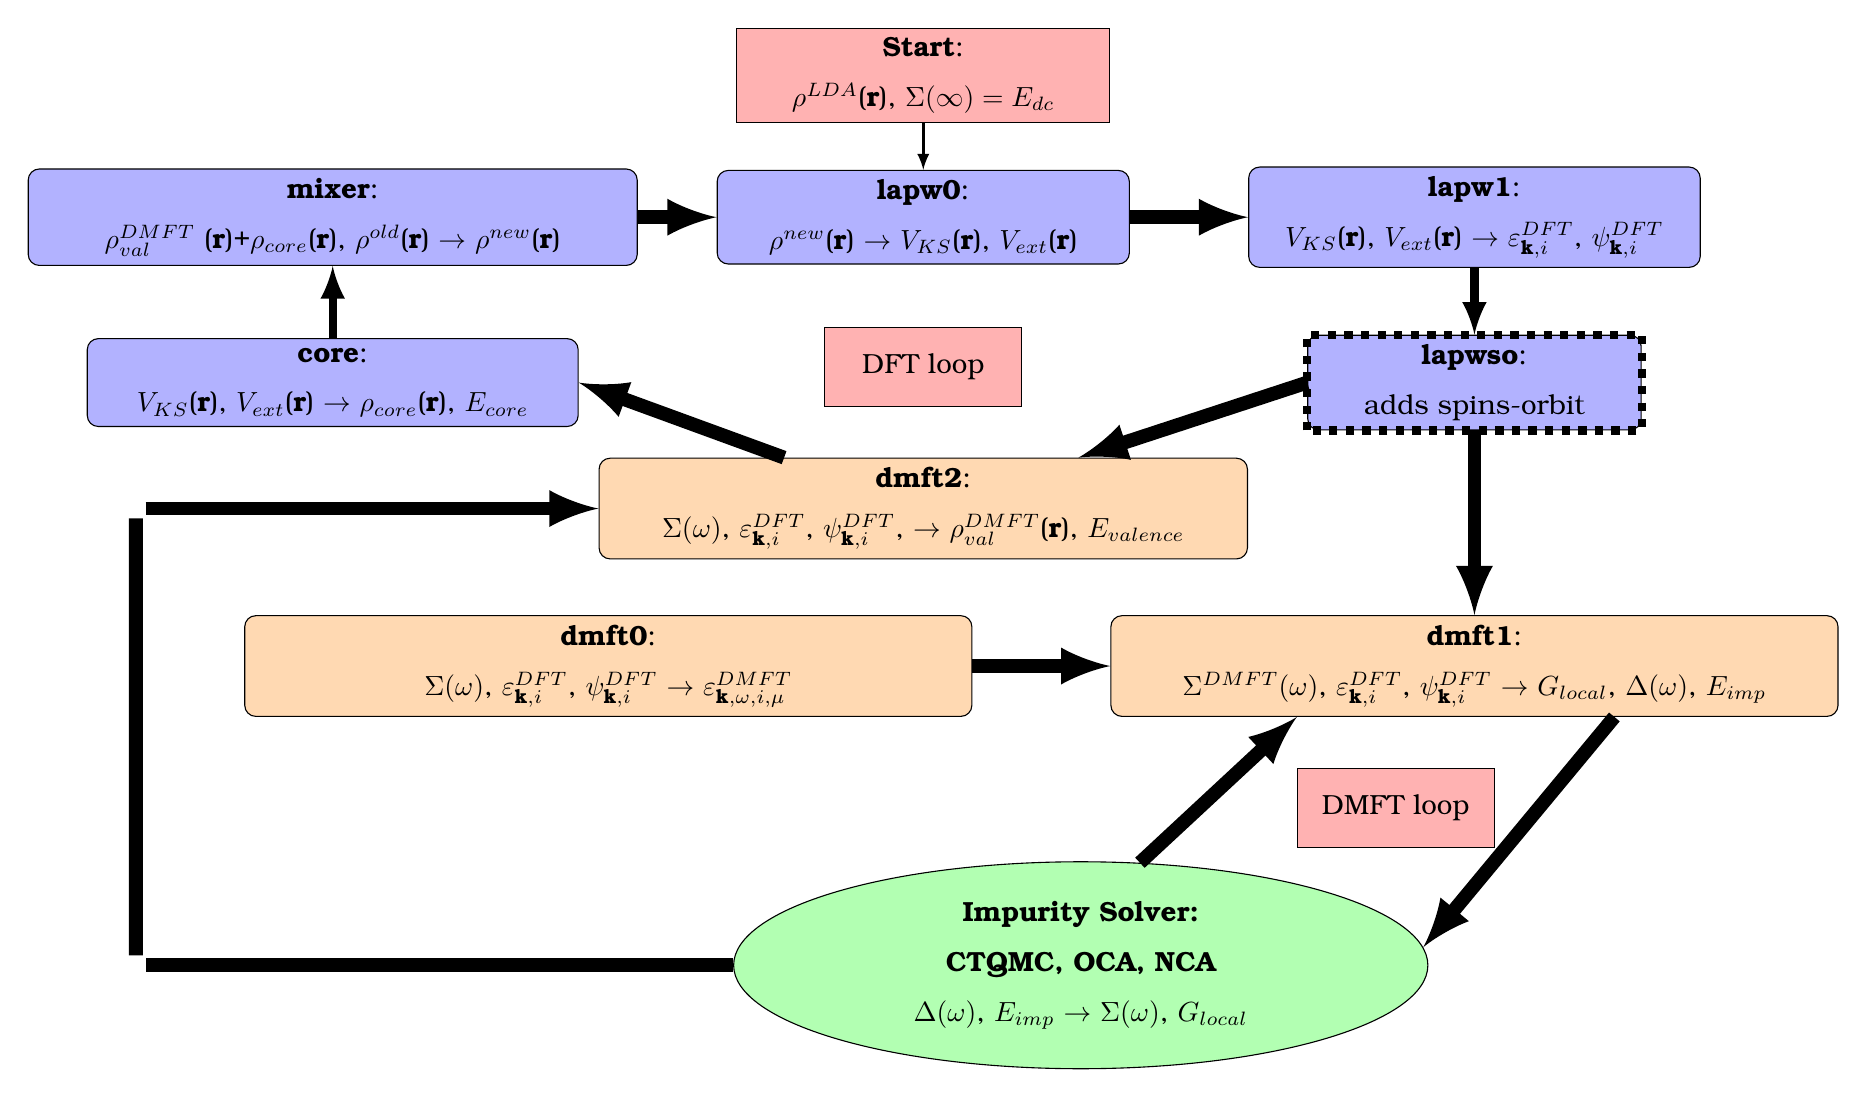
\begin{tikzpicture}[node distance=1.8cm]
    \linespread{1.5}

    \node(Start)[DFT_DMFT]{\parbox{4.5cm}{\centering \textbf{Start}:\\ $\rho^{LDA}$(\textbf{r}), $\Sigma(\infty)=
E_{dc}$}};

    \node(DFT0)[DFT, below of=Start]{\parbox{5cm}{\centering \textbf{lapw0}:\\ $\rho^{new}$(\textbf{r}) $\rightarrow$ 
$V_{KS}$(\textbf{r}), $V_{ext}$(\textbf{r})}}
	  edge[arrow, <-, line width=1pt](Start);

    \node(DFT1)[DFT, below of=Start, xshift=7cm]{\parbox{5.5cm}{\centering \textbf{lapw1}:\\ $V_{KS}$(\textbf{r}), 
$V_{ext}$(\textbf{r}) $\rightarrow$ $\varepsilon^{DFT}_{\textbf{k},i}$, $\psi^{DFT}_{\textbf{k},i}$}}
	  edge[arrow, <-](DFT0);

    \node(DFT5)[DFT, below of=Start, xshift=-7.5cm]{\parbox{7.5cm}{\centering \textbf{mixer}:\\ $\rho^{DMFT}_{val}$
(\textbf{r})+$\rho_{core}$(\textbf{r}), $\rho^{old}$(\textbf{r}) $\rightarrow$ $\rho^{new}$(\textbf{r})}}
	  edge[arrow](DFT0);

    \node(DFT)[DFT_DMFT, below of=DFT0, yshift=-0.1cm]{DFT loop};

    \node(DFT2)[DFT, below of=DFT1, yshift=-0.3cm]{\parbox{4cm}{\centering \textbf{lapwso}:\\ adds spins-orbit}}
	  edge[arrow, <-, line width=3pt](DFT1);
	  \draw[dashed, line width=3pt](DFT2.south west) rectangle (DFT2.north east);

    \node(DFT4)[DFT, below of=DFT5, yshift=-0.3cm]{\parbox{6cm}{\centering \textbf{core}:\\ $V_{KS}$(\textbf{r}), 
$V_{ext}$(\textbf{r}) $\rightarrow$ $\rho_{core}$(\textbf{r}), $E_{core}$}}
	  edge[arrow, line width=3pt](DFT5);

    \node(DMFT2)[DMFT, below of=DFT]{\parbox{8cm}{\centering \textbf{dmft2}:\\ $\Sigma(\omega)$, $\varepsilon^{DFT}_
{\textbf{k},i}$, $\psi^{DFT}_{\textbf{k},i}$, $\rightarrow$ $\rho^{DMFT}_{val}$(\textbf{r}), $E_{valence}$}}
	  edge[arrow](DFT4.east)
	  edge[arrow, <-](DFT2.west);

    \node(DMFT1)[DMFT, below of=DMFT2, yshift=-0.2cm, xshift=7cm]{\parbox{9cm}{\centering \textbf{dmft1}:\\ 
$\Sigma^{DMFT}(\omega)$, $\varepsilon^{DFT}_{\textbf{k},i}$, $\psi^{DFT}_{\textbf{k},i}$ $\rightarrow$ $G_{local}$, 
$\Delta(\omega)$, $E_{imp}$}}
	  edge[arrow, <-](DFT2);

    \node(DMFT0)[DMFT, below of=DMFT2, yshift=-0.2cm, xshift=-4cm]{\parbox{9cm}{\centering \textbf{dmft0}:\\ 
$\Sigma(\omega)$, $\varepsilon^{DFT}_{\textbf{k},i}$, $\psi^{DFT}_{\textbf{k},i}$ $\rightarrow$ $\varepsilon^
{DMFT}_{\textbf{k},\omega,i,\mu}$}}
	  edge[arrow](DMFT1);

    \node(DMFT)[DFT_DMFT, below of=DMFT2, yshift=-2cm, xshift=6cm]{DMFT loop};

    \node(empty1)[below of=DMFT, yshift=-0.2cm, xshift=-16cm]{};

    \node(empty2)[below of=DFT4, yshift=0.2cm, xshift=-2.5cm]{}
	  edge[arrow, -](empty1)
	  edge[arrow](DMFT2);

    \node(Impurity)[impurity, below of=DMFT, xshift=-4cm, yshift=-0.2cm]{\parbox{6cm}{\centering \textbf{Impurity 
Solver:\\ CTQMC, OCA, NCA}\\ $\Delta(\omega)$, $E_{imp}$ $\rightarrow$ $\Sigma(\omega)$, $G_{local}$}}
	  edge[arrow, -](empty1);

    \path (DMFT1.340) edge[arrow] (Impurity.3);
    \path (Impurity.60) edge[arrow] (DMFT1.196);

    \end{tikzpicture}

  \end{figure}

  \end{landscape}

  \cleardoublepage

  \part{Installation}

  \bigskip
  For detailed information about how to download, properly install and configure the \emph{WIEN2k} source code for 
DFT calculations (version WIEN2k\_14.1, please refer to \emph{WIEN2k User's Guide, WIEN2k\_14.1}. 

  \url{http://www.wien2k.at}

  Furthermore, below illustrates how to properly install and configure the \emph{DMFT-Wien2K} source code for DMFT 
calculations (version 2012). 

  The program consists of many independent programs and executables, which are written in C++, fortran 90 and Python. 
Before you start the installation, you must make sure that the following packages are installed in the system.

{\color{cyan}
  \begin{itemize}

  \item intel mkl library

  \item gnu C++ compiler

  \item intel fortran compiler or gnu fortran compiler

  \item gsl library: gnu scientific library

  \item Python with numpy and scipy

  \item Python CXX package

  \end{itemize}
}

  Except for some Python packages, these are quite standard codes, which are likely already installed.

  The compilation consists of six simple steps:

{\color{cyan}
  \begin{itemize}

  \item download the code here: 

  \url{http://hauleweb.rutgers.edu/downloads/}, 

  unpack it (\textbf{tar xzvf dmft\_w2k.tgz}) and cd to directory main.

  \item Edit the file \emph{Makefile.in} under the main directory to set the path to compilers on the system, their 
options, and libraries (see description below)

  \item set the environment variable \emph{WIEN\_DMFT\_ROOT} (in ~/.bashrc) to point to the directory you plan to 
install the binaries code

  \item type \textbf{make}

  \item type \textbf{make install}

  \item for execution, also make sure that the following variables are properly set in \emph{.bashrc}:

    \begin{itemize}

    \item WIENROOT : should be set during \emph{WIEN2k} installation to \emph{WIEN2k} executables.

    \item PATH=\$WIENROOT:\$WIEN\_DMFT\_ROOT:\$PATH : add both dmft and wien executables to your path.

    \item PYTHONPATH= :\$WIEN\_DMFT\_ROOT: :\$PYTHONPATH : add dmft binary dir to PYTHONPATH.

    \item OMP\_NUM\_THREADS=$<n>$ : you might want to set number of cores for multithreading. Note that dmft1 and 
dmft2 steps support multithreading. ctqmc uses only mpi (which is very efficient in Monte Carlo). For ctqmc, it is 
best to have OMP\_NUM\_THREADS=1 to avoid collision between independent Monte Carlo walkers parallelized by MPI. For 
dmft1 and dmft2 steps, one can use double parallelization: k-point parallelization with MPI and extra parallelization 
with open\_mpi, setting OMP\_NUM\_THREADS to number of cores on a node. For non-experts, set OMP\_NUM\_THREADS=1.

    \item EDITOR : environment variable EDITOR should be set (during WIEN2k installation) to preferred editor, for 
example ``emacs -nw'' or ``vi''.

    \item SCRATCH : environment variable SCRATCH should be set to current dir, i.e., \emph{export SCRATCH=./}

    \end{itemize}

  \end{itemize}
}

  Here we will briefly describe the options which are set in \emph{Makefile.in} and might need to be changed. Note 
that this file \emph{Makefile.in} is included in all other makefiles located in subdirectories (there are around 
20 makefiles in total), hence no other makefile needs to be edited.

  \emph{Makefile.in} contains:

{\color{cyan}
  \begin{itemize}

  \item DESTDIR = \$ (WIEN\_DMFT\_ROOT) : Here we expect that environment variable \$WIEN\_DMFT\_ROOT is set on the 
system (likely in .bashrc).

  \item F90 = ifort : non parallel version of fortran compiler, which is used to compile smaller modules.

  \item F77 = ifort : some older modules need non-parallel fortran77 compiler. 

  \item preproc = cpp : preprocessor, which ca preprocess source code (in this case fortran files).

  \item WFOPT = -xHOST -03 -ipo -no-prec-div -traceback -FR -override-limits -openmp -I\$(MKLROOT)/include/intel64/
lp64 -I\$(MKLROOT)/include : fortran options for both dmft1 (ksum) and dmft2 (chargesc) codes. More detailed 
explanation of some options.

    \begin{itemize}

    \item -03 -override-limits -pad -mavx : These options are for maximal optimization, regardless of memory required, 
and using intels avx technology, etc... These options most likely need some changes on different platforms.

    \item -pre\_div -mpl -pc80 : controls floating point precision. Might need to be changed.

    \item -FR : is needed to tell compiler that fortran code is written in free format even when extension of files 
is ``.f''.

    \item -openmp : the code is using multi-threading techniques, hence it is wise to enable them.

    \item -DINTEL\_VML defines to use Intel's vector math library (if available).

    \end{itemize}

  \item FFLAGS = -O3 -fPIC : similar fortran options than above. These are used in some fortran codes which are packed 
into python modules (.so) and they need extra option ``-fPIC''. This option ensures position independent code, which 
can be packed into shared libraries.

  \item C++ = icpc : both g++ and intel icpc should work here. It is used for smaller impurity modules.

  \item OFLAGS = -O3 : options for C++ compiler for these small impurity modules.

  \item GFLAGS = -g -C : options for C++ compiler for these small impurity modules.

  \item CMP = f2py --fcompiler=intelem : name of the fortran to python converter. The option ``--fcompiler=intelem'' 
might need to be changed, because it depends on the platform.

  \item WLDFLAGS = -i-static \$(FOPT) : linking flags for many fortran codes, such as dmft1 step. 

  \item WLIBS = -L\$(MKLROOT)/lib/intel64 \$(MKLROOT)/lib/intel64/\\libmkl\_blas95\_lp64.a \$(MKLROOT)/lib/intel64/
libmkl\_lapack95\_lp64.a

  -lmkl\_cdft\_core -lmkl\_intel\_lp64 -lmkl\_intel\_thread -lmkl\_core
  
  -lmkl\_blacs\_intelmpi\_lp64 -liomp5 -lpthread -lm 

  : linking options for dmft2 steps, which does not use WLDFLAGS, and also requires intel math library.

  \item PFLAGS = -D\_MPI -DMPICH\_IGNORE\_CXX\_SEEK -I/home/user/gsl/include : compilation flags for ctqmc code 
compiled with PC++. Here ``-D\_MPI'' enables parallel version, ``-DMPICH\_IGNORE\_CXX\_SEEK'' avoids some name-conflict 
between mpich and standard libraries. The rest of the options are for optimization.

  \item PC++ = mpicxx : parallel C++ compiler used for compiling ctqmc code.

  \item pcc = mpicc : parallel c-compiler

  \item PLIBS = -L\$(MKLROOT)/lib/intel64 \$(MKLROOT)/lib/intel64/

  libmkl\_blas95\_lp64.a \$(MKLROOT)/lib/intel64/libmkl\_lapack95\_lp64.a

  -lmkl\_cdft\_core -lmkl\_intel\_lp64 -lmkl\_intel\_thread -lmkl\_core

  -lmkl\_blacs\_intelmpi\_lp64 -liomp5 -lpthread -lm -L/home/rcohen/lib

  -L/share/apps/intel/impi/4.0.1.007/intel64/lib -lmpich -lgsl 

  : linking options for ctqmc. We need gsl library for random number generator.

  \item LLIBS = -L\$(MKLROOT)/lib/intel64 \$(MKLROOT)/lib/intel64/

  libmkl\_blas95\_lp64.a \$(MKLROOT)/lib/intel64/libmkl\_lapack95\_lp64.a

  -lmkl\_cdft\_core -lmkl\_intel\_lp64 -lmkl\_intel\_thread -lmkl\_core

  -lmkl\_blacs\_intelmpi\_lp64 -liomp5 -lpthread -lm

  -L/share/apps/intel/impi/4.0.1.007/intel64/lib -lmpich

  : linking options for other C++ utility modules.

  \item CMPLIBS = --opt='-fast' --link-lapack\_opt : options for f2py compiler. We need to link lapack and blas to 
several f2py modules.

  \item CMPLIBS2 = --f90flags='-openmp ' --opt='-fast' --link-lapack\_opt : some python modules written in fortran 
can support multithreading, hence we allow openmp.

  \end{itemize}
}

Note: When installing numpy on a linux distribution, make sure to use gnu c++ compiler (as opposed to intel c++ 
compiler). Before installing numpy and scipy, you should set environment variables CC and CXX to CC=gcc and CXX=g++. 
Otherwise, f2py might use intel c++ compiler (icc and icpc), which does NOT work properly in some versions of python. 
\citep {Haule2010}

%  \hyperlink{my toc}{Back to Table of Contents}

  \newpage
  \part{\texorpdfstring{General steps for running self-consistent cycles in DFT + DMFT}{General steps for 
running self-consistent cycles in DFT + DMFT}}

    \section{DFT part}

      \subsection{Prepare struct-files}

	\subsubsection{Gather all the required information}

	  \begin{itemize}

	    \item  The lattice parameters,

  lengths a, b, c in Bohr or \AA{ngstrom} and angles $\alpha$, $\beta$, $\gamma$.

	    \item  The space group according to the ``International Tables for Crystallography'', 
  
  \url{http://it.iucr.org/}.

	    \item  The positions of all equivalent atoms (number them 1, 2, 3, ..., e.g., Fe 1, Fe 2, if there are 
many) and the positions of all inequivalent atoms in fractions of the unit cell. Alternatively you can utilize 
\emph{StructGen} in WIEN2k to generate all the equivalent positions automatically by providing only the inequivalent 
positions and the space group.

	  \end{itemize}

	\subsubsection{Generate struct-files}

  A new struct-file should be generated on which we can run DFT and DMFT calculations. There are many approaches, 
such as by hand (using a simple command, converting other files into struct-files and manipulating example 
struct-files) and by using \emph{w2web}.

  \begin{itemize}[leftmargin=0.2in]
    
    \item Use a simple command, \emph{makestruct\_lapw}

  In the newest version of WIEN2k, i.e., WIEN2k\_14.1, we can easily create struct-files by a simple command shown 
below and then interactively type in all the required input information.

  ``\textbf{makestruct\_lapw}''

  Note that this command can only generate a struct-file named \emph{init.struct}. Copy it to your desired name
 \emph{case.struct} by the command, 

  ``\textbf{cp init.struct case.struct}''

  Also, please be reminded that \emph{makestruct\_lapw} command is only suitable for small to medium sized 
cells. For large sized cells, \emph{cif2struct} is recommended which will be introduced next.

  \cleardoublepage

    \item Convert other files into struct-files using \emph{cif2struct}

  Besides the \emph{makestruct\_lapw} command, converting established \emph{.cif, .txt} files into \emph{.struct} 
files is sometimes more convenient. 

  Store structural data in \emph{case.cif} or \emph{case.txt} files, then convert them into the
 \emph{case.struct} files using the commands,

  ``\textbf{cif2struct case.cif}'' or 

  ``\textbf{cif2struct case.txt}''

  Some \emph{.cif} files are available for download from Crystallographic databases (e.g., the Inorganic Crystal 
Structure DataBase).

  \url{http://it.iucr.org/}) 

  \emph{.txt} files can be created by hand. Type in the following command to make a new \emph{.txt} file.

  ``\textbf{vi case}''

  Make sure that the \emph{.txt} file contains all the data in the correct format, and one example of the contents of
 the \emph{.txt} file is given below, (see Table \ref{Example .txt file to be converted into .struct file})

  \begin{table}[ht]
    \centering
    \caption{Example \emph{.txt} file to be converted into \emph{.struct} file}
    \label{Example .txt file to be converted into .struct file}
    \vspace{2ex}

  \begin{tabular}{|l|l|l|l|l|l|l|}

  \hline
  \textbf{b}		&			&			&	&	& 		& ``a..Ang, 
b..Bohr''\\ \hline

  \textbf{0.0} 		& \textbf{0.0} 		& \textbf{0.0}		&	&	& 		& ``shift of 
origin''\\ \hline

  \textbf{8.1450} 	& \textbf{8.1450} 	& \textbf{8.1450} 	& \textbf{90} 	& \textbf{90} 	& \textbf{90}
	& ``a, b, c, angles $\alpha, \beta, \gamma$''\\ \hline

  \textbf{Fm-3m}	&			&			&	&	&		& 
``space-group symbol''\\ \hline

  \textbf{Fe}		&			&			&	&	&		& ``atom-
name''\\ \hline

  \textbf{0.0000000} 	& \textbf{0.0000000} 	& \textbf{0.0000000}	&	&	&		& ``atomic
 position''\\ \hline

  \end{tabular}

  \end{table}

  \cleardoublepage

    \item Manipulate existing example struct-files

  When the elements in the compounds are very similar and presumably the unit cell structures are quite similar, it 
is also acceptable to make some minor modifications on the parameters in the existing example struct-files. You can 
find and download some example struct-files in the installed WIEN2k folder, i.e., \emph{example\_struct\_files} 
folder, or from the \emph{Input Files/struct} column on Haule's website, 

  \url{http://hauleweb.rutgers.edu/database\_w2k/}

  \cleardoublepage

    \item Use \emph{w2web} to set up struct-files

  The new interface \emph{w2web} provides a more user-friendly environment to make struct-files and derive some 
properties thereafter. 

  For the first-time user, set up your username and password by the command,  

  ``\textbf{w2web -p xxxx}''

  in which ``xxxx'' stands for the default port number (7890) or a different port number between 1024 and 65536. 

  If you forget your portnumber, simply use the command,

  ``\textbf{ps -ef $|$ grep w2web}''

  If the remote server machine, e.g., \emph{mw}, does not have the browser installed, you can establish a tunnel 
between \emph{mw} server and your local server by the command, 

  ``\textbf{ssh -X -L 5890:localhost:7890 mw}''

  In the above case, \emph{7890} and \emph{5890} are considered as port 1 on the \emph{mw} side and port 2 on the 
local side (any random number you want) respectively. Once the tunnel is established, you can start using \emph{w2web}
 interface by opening your local browser, e.g., \emph{firefox}, and typing in the following address and your username
 and password,

  ``\textbf{username@localhost:5890}''

  In the \emph{w2web} interface, there are three steps to set up the session part. The first step is to \emph{Create 
new session} if you don't have one, choose your session name (\emph{case}) and click \emph{Create}. The second step 
is to change into or create a new directory in which all your output files will be stored, and click \emph{Select 
current directory}. The last step is to click \emph{Click to restart session}, and the main window of \emph{w2web} 
will show up. (see Figure \ref{Main window of w2web})

  \begin{figure}[h]
    \centering
    \caption{Main window of \emph{w2web}}
    \label{Main window of w2web}
    \vspace{2ex}
    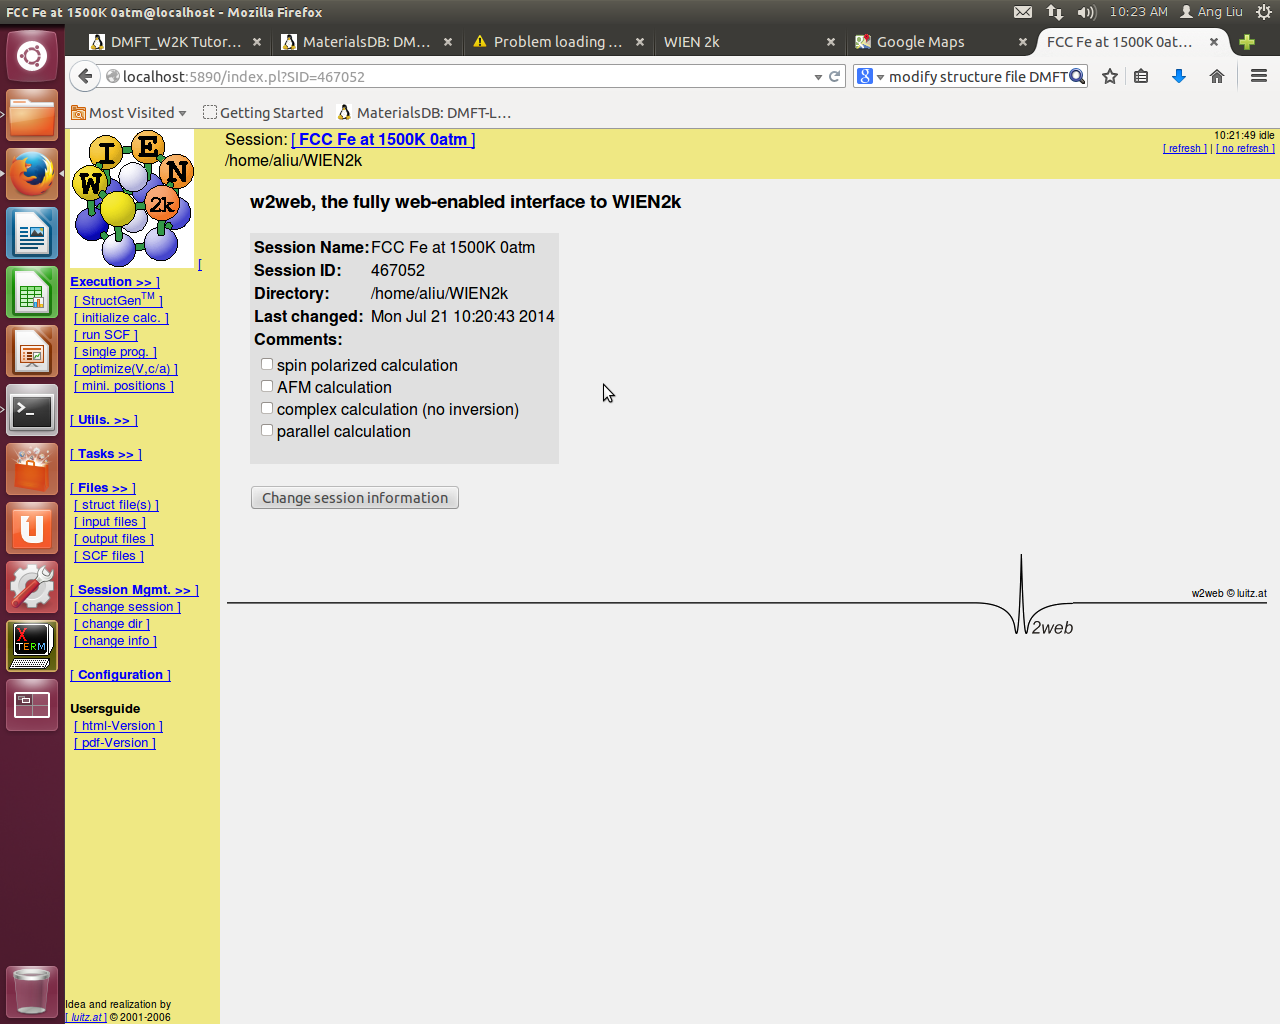
\includegraphics[scale=0.35, trim=2.3cm 0cm 0cm 4.3cm, clip=true]{Mainwindow}
  \end{figure}

  On the left side of the \emph{w2web} main window, start the struct-file generator by clicking on 
\emph{$StructGen^{TM}$} under the directory \emph{Execution $>>$}. It will ask for the necessary information to 
create \emph{case.struct}. The questions asked and some actions taken are listed below,

    \begin{itemize}

      \item Please specify the number of independent atoms of your initial structure

      \item Click \emph{Generate template}

      \item Title

      \item Lattice Type

      \item Lattice parameters (lengths: a, b, c in \AA{} or bohr) (angles: $\alpha$, $\beta$, $\gamma$)

      \item Inequivalent Atoms:

	  Atom n: Atom-name

	  Pos n: Atomic position of atom n (see Figure \ref{StructGen screen before clicking ``Save Structure''})

  \begin{figure}[h]
    \centering
    \caption{\emph{StructGen} screen before clicking ``Save Structure''}
    \label{StructGen screen before clicking ``Save Structure''}
    \vspace{2ex}
    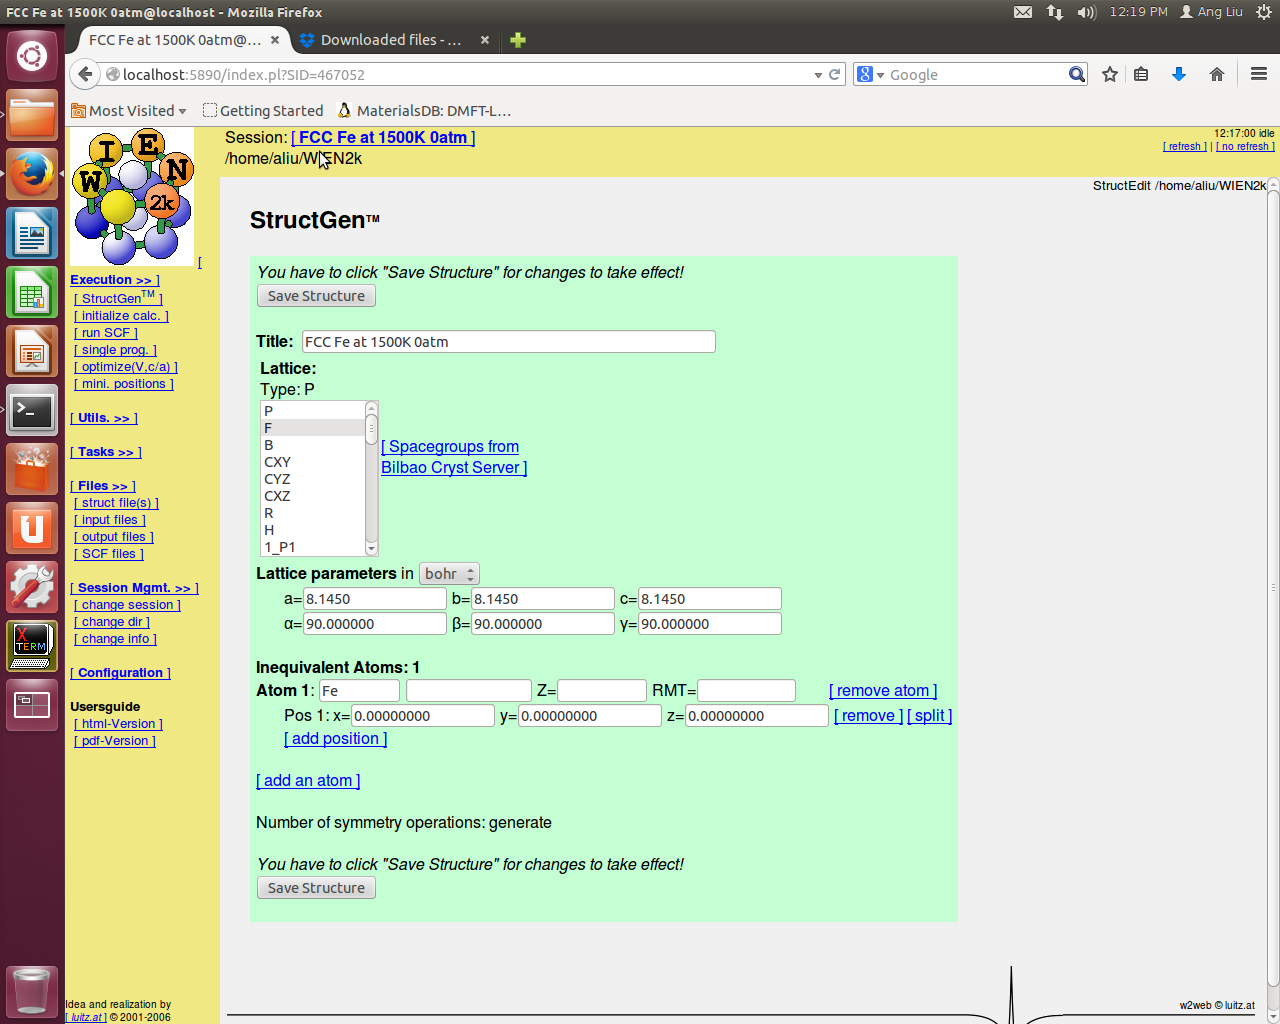
\includegraphics[scale=0.35, trim=2.3cm 0cm 0cm 4.3cm, clip=true]{StructGen2}
  \end{figure}

  \cleardoublepage

      \item Click \emph{Save Structure}

      \item Click \emph{set automatically RMT and continue editing (do it at least once!)} (RMT: muffin-tin radius, 
atomic sphere radius) (see Figure \ref{Choosing options for Automatic determination of Radius of Muffin-Tin (RMT)})

  \begin{figure}[ht]
    \centering
    \captionsetup{justification=centering}
    \caption{Choosing options for Automatic determination of Radius of Muffin-Tin (RMT)}
    \label{Choosing options for Automatic determination of Radius of Muffin-Tin (RMT)}
    \vspace{2ex}
    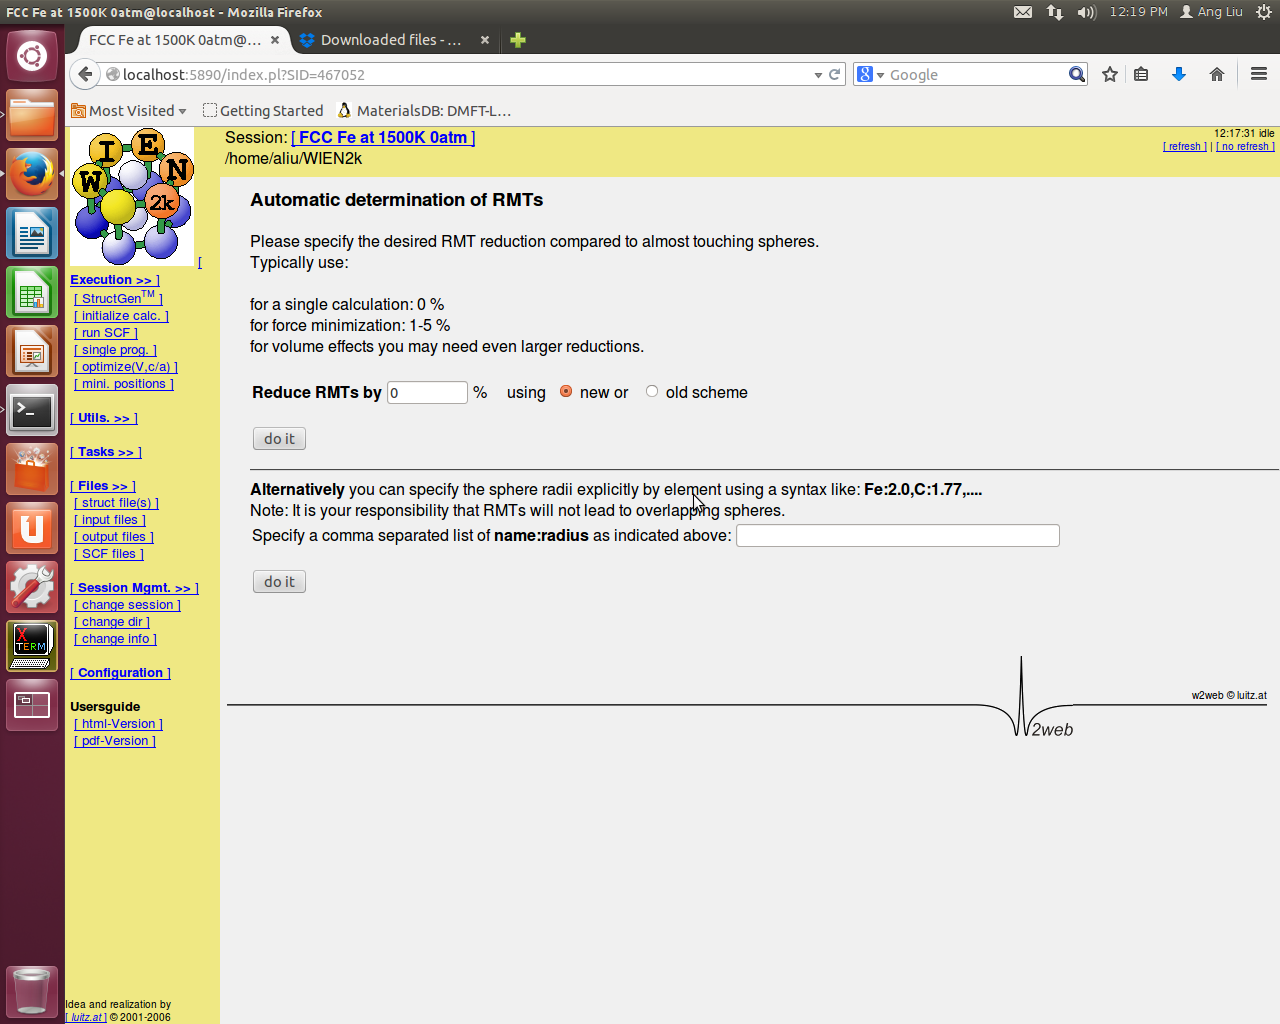
\includegraphics[scale=0.35, trim=2.3cm 0cm 0cm 4.3cm, clip=true]{StructGen3}
  \end{figure}

  \cleardoublepage

      \item Click \emph{do it!} (Z and RMT values will be calculated automatically for each atom) (figure 
\ref{StructGen screen after saving})

  \begin{figure}[ht]
    \centering
    \caption{\emph{StructGen} screen after saving}
    \label{StructGen screen after saving}
    \vspace{2ex}
    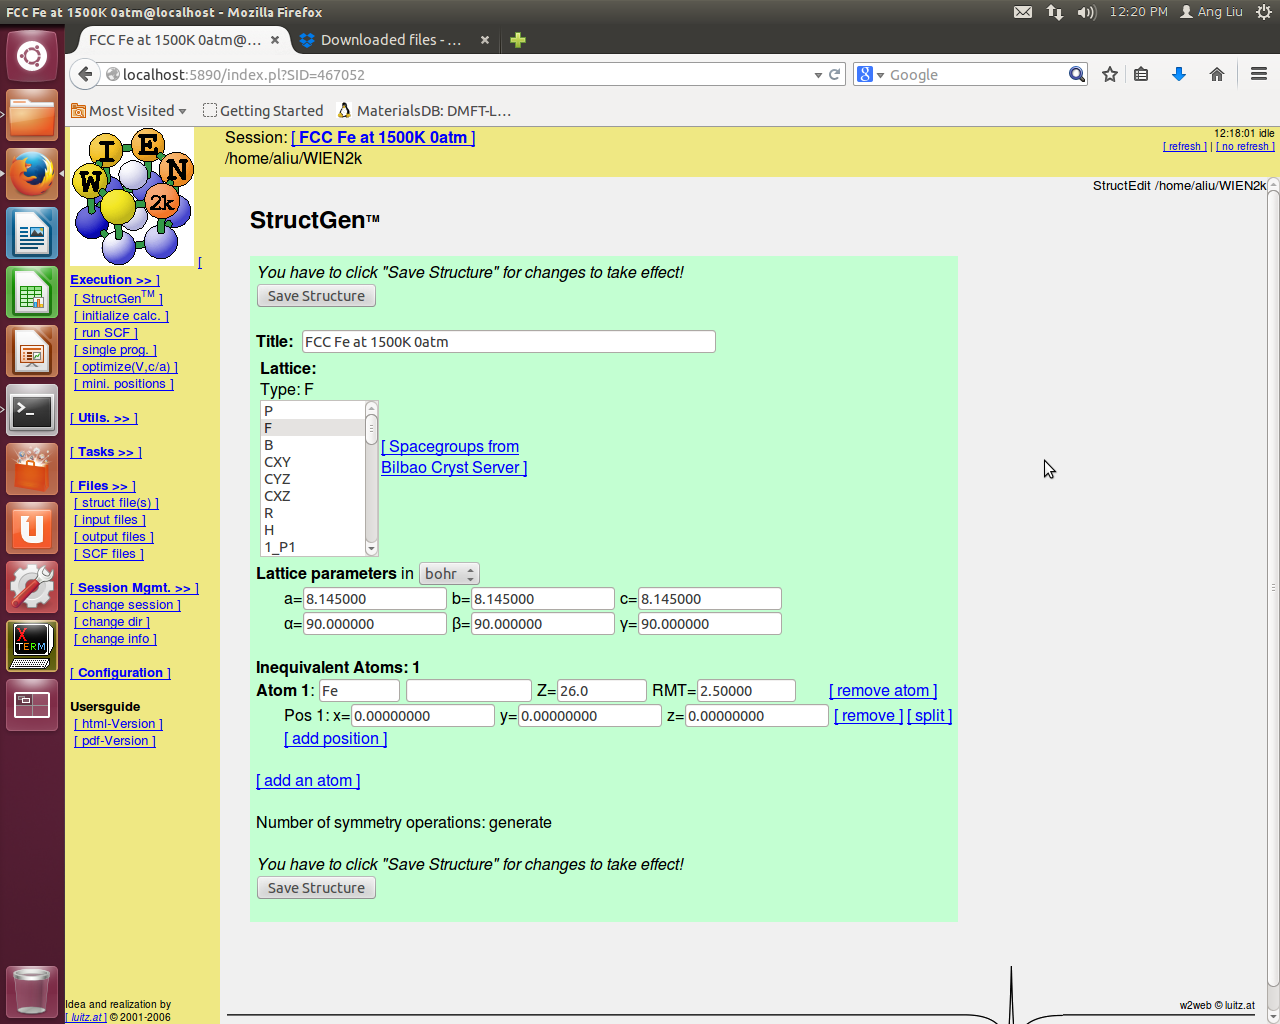
\includegraphics[scale=0.35, trim=2.3cm 0cm 0cm 4.3cm, clip=true]{StructGen4}
  \end{figure}

  \cleardoublepage

      \item Click \emph{Save Structure}

      \item Click \emph{save file and clean up (when you are done)} (View only mode of Struct-file will show up) 
(see Figure \ref{StructGen screen after cleaning up})

  \begin{figure}[ht]
    \centering
    \caption{\emph{StructGen} screen after cleaning up}
    \label{StructGen screen after cleaning up}
    \vspace{2ex}
    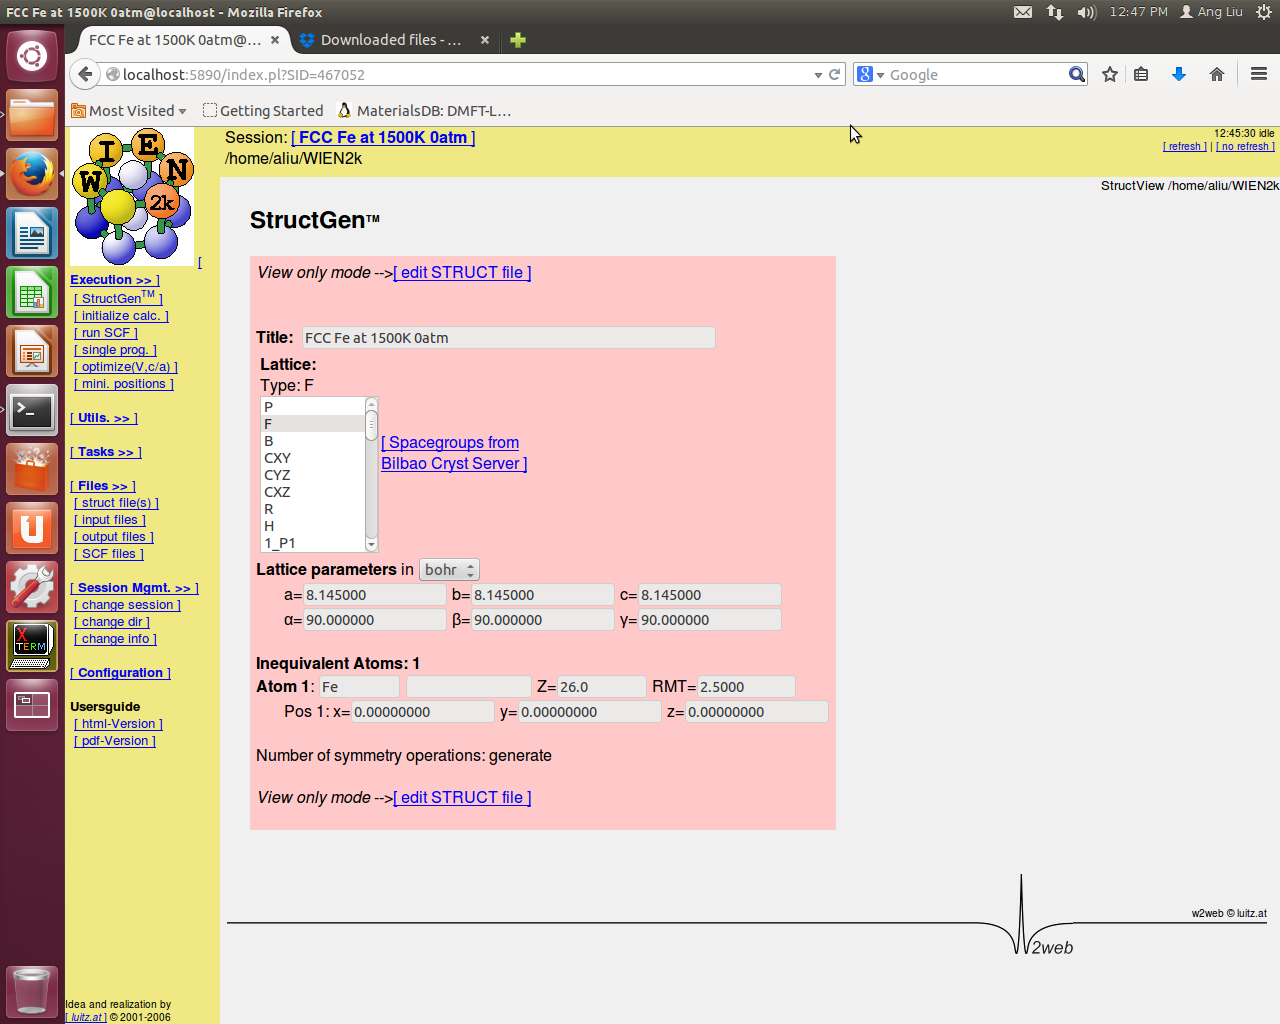
\includegraphics[scale=0.35, trim=2.3cm 0cm 0cm 4.3cm, clip=true]{StructGen5}
  \end{figure}

    \end{itemize}
  
  To double check if your \emph{case.struct} is in your specified directory, go to \emph{show all files} under the 
directory \emph{Files $>>$}. 

  \item One example of \emph{.struct} file

  Below illustrates the head part of one example of the generated struct-file for FCC Fe. (see Table
 \ref{Head of example struct-file generated for FCC Fe})

  \cleardoublepage

  \begin{landscape}

  \begin{table}[ht]
  \centering
  \caption{Head of example struct-file generated for FCC Fe}
  \label{Head of example struct-file generated for FCC Fe}

{\color{cyan}

  \resizebox{1.32\textwidth}{!}{

  \begin{tabular}{llllll}

  FCC Fe			&			&		&		&		&	\\

  F LATTICE,NONEQUIV.ATOMS	& 			& 1		& 225		& Fm-3m		&	\\

  MODE OF CALC=RELA unit=bohr	&			&		&		&		&	\\

  8.145000			& 8.145000		& 8.145000	& 90.00		& 90.00		& 90.00	\\

  ATOM 1:			& X=0.0000		& Y=0.0000	& Z=0.0000	&		&	\\

  				& MULT= 1		& ISPLIT= 2	&		&		&	\\

  Fe				& NPT= 781		& R0=.000050	& RMT= 2.5000	& Z: 26.000	&	\\

  LOCAL ROT MATRIX:		& 1.00000		& 0.00000	& 0.00000	&		&	\\

				& 0.00000		& 1.00000	& 0.00000	&		&	\\

				& 0.00000		& 0.00000	& 1.00000	&		&	\\

48 NUMBER OF SYMMETRY OPERATIONS& 			&		&		&		&	\\

  1				& 0			& 0		& 0.000		&		&	\\

  0				& -1			& 0		& 0.000		&		&	\\

  0				& 0			& -1		& 0.000		&		&	\\

				&			&		& 1		&		&	\\

  \end{tabular}
}

}

  \end{table}

 \end{landscape}

    \end{itemize}
  \cleardoublepage

      \subsection{Initialize DFT calculations using init\_lapw}

  \emph{case.struct} file contains all the information needed for the DFT calculations of the crystal structures.
 Run the following command, 

  ``\textbf{init\_lapw}''

  The following shows all the subsequent questions and corresponding answer choices.

  \begin{enumerate}

   \item The screen first shows:

  next is setrmt. 

  Automatic determination of RMTs. Please specify the desired RMT reduction compared to almost touching spheres.

  Typically, for a single calculation just hit enter, for force minimization use 1-5; for volume effects you may 
need even larger reductions. 

   \item Answers choices to a series of questions,

    \begin{enumerate}

  \item Use old or new scheme (o/N)

  \item accept these radii; discard them; or rerun setRmt (a/d/r) 

  \item nn-bondlength factor (usually=2)

  \item continue with sgroup or edit the case.struct file (c/e) 

  \item continue with symmetry (old case.struct) or use/edit case.struct\_sgroup (c/e) 

  \item continue with lstart or edit the case.struct\_st file (c/e/x)

  \item Eventually specify switches for instgen\_lapw (or press ENTER): -up (default) -dn -nm (non-magnetic) -ask 

  \item SELECT XCPOT, 13:PBE-GGA (Perdew\_Burke-Ernzerhof 96) 5:LSDA 11:WC-GGA (Wu-Cohen 2006) 19:PBEsol-GGA 
(Perdew etal.2008)

  \item SELECT ENERGY to separate core and valence states: -6.0 Ry (check how much core charge leaks out of
 MT-sphere)

  \item continue with kgen or edit the case.inst file and rerun lstart (c/e)

  \item number of k-points in whole cell, usually 200-500 

  \item continue with dstart or execute kgen again or exit (c/e/x)

  \item do you want to perform a spinpolarized calculation (n/y)

    \end{enumerate}
     
  \end{enumerate}

  \cleardoublepage

      \subsection{Run the self-consistency cycles (SCF) of DFT calculations}

  After \emph{init\_lapw}, there are many new files generated in the \emph{case} folder. The next step is 
to run self-consistency cycles (SCF) of DFT calculations. It is strongly suggested to submit the DFT calculations 
job via \emph{submit\_dft.scr} script utilizing services provided by a parallel computing machine (e.g., \emph{mw}
 server). An example of \emph{submit\_dft.scr} file is shown below,

{\color{cyan}

  \#!/bin/bash

  \#\$ -N /test

  \#\$-S /bin/bash

  \#\$-cwd

  \#\$-j y

  \#\$-r no

  \#\$-m abes

  \#\$-M user@carnegiescience.edu

  \#\$-pe mpi 8

  \#\$-P GL

  \#\$-l vf=2G

  \#\$-l h\_vmem=2G

  ulimit -l unlimited

  . /home/user/.bashrc

  pwd

  \#\#\#echo ``env mpirun --verbose -n 4 '' $>$ mpi\_prefix.dat

  echo \$jobdir

  export HOME=/san2/user

  \#\#\#export TMPDIR=/san3/smandal/main\_July\_2012

  export OMP\_NUM\_THREADS=2

  set -x

  pwd

  echo \$jobdir

  export OMP\_NUM\_THREADS=2

  env

  cat \$PE\_HOSTFILE

  let n='mkmachinefile.sh \$PE\_HOSTFILE'

  cat .machines

  echo n=\$n

  \#\#\#export MY\_NSLOTS=\$n

  echo ``env OMP\_NUM\_THREADS=1 mpirun -n 8 '' $>$ mpi\_prefix.dat

  echo ``env OMP\_NUM\_THREADS=1 mpirun -n \$n '' $>$ mpi\_prefix.dat2

  \#which mpirun

  /share/apps/intel13/composer\_xe\_2013.0.079/bin/compilervars.sh intel64

  \#export INTEL\_LICENSE\_FILE=27000@troy.tacc.utexas.edu

  \#echo \$\{INTEL\_LICENSE\_FILE\}

  \#ls -l /etc/redhat -release

  \$WIENROOT/run\_lapw -p
}

  The command to submit the DFT calculation job to \emph{mw} server is as follows,

  ``\textbf{qsub submit\_dft.scr}''
 
  Another way to run SCF is to use the command ``\textbf{run\_lapw}'', but it is not recommended.

  The self-consistency cycles (SCF) consist of the following parts:

  \emph{LAPW0} (POTENTIAL) generates potential from density

  \emph{LAPW1} (BANDS) calculates valence bands (eigenvalues and eigenvectors)

  \emph{LAPW2} (RHO) computes valence densities from eigenvectors

  \emph{LCORE} computes core states and densities

  \emph{MIXER} mixes input and output densities

  After SCF of DFT calculations, good charge densities have been converged. You can save your results by the 
command ``\textbf{save\_lapw}''.   

  
  \cleardoublepage

    \section{DMFT part}

      \subsection{Initialize DMFT calculations}

  Following \emph{init\_lapw} and SCF of DFT, proceed to the command,

  ``\textbf{init\_dmft.py}''

  to invoke DMFT calculations in the current directory.

  Answer choices thereafter are shown below, 

  \begin{itemize}

    \item Specify correlated atoms (e.g. 1-4, 7, 8):

    \item Do you want to continue; or edit again? (c/e):

    \item For each atom, specify correlated orbital(s) (e.g. d, f):

    \item Do you want to continue; or edit again? (c/e):

    \item Specify qsplit for each correlated orbital (default = 0):  

    \item Do you want to continue; or edit again? (c/e):

    \item Do you want to group any of these orbitals into cluster-DMFT problems? (y/n):

    \item Enter the correlated problems forming each unique correlated problem, separated by spaces (e.g. 
1, 3 2, 4 5-8):

    \item Do you want to continue; or edit again? (c/e):

    \item Broken symmetry run? (y/n):

    \item Range (in eV) of hybridization taken into account in impurity problems; default -6.0, 6.0: -10, 10:

    \item Perform calculations on real; or imaginary axis? (r/i):

    \item Is this a spin-orbit run? (y/n):

    \item Generate blank sig.inp? (y/n):

  \end{itemize}

  \cleardoublepage

      \subsection{Prepare all files}

	\subsubsection{Prepare input files (case.indmfl, case.indmfi) and output files}

  The initialization of DMFT calculations by \emph{init\_dmft.py} will generate two input files, \emph{case.indmfi} 
and \emph{case.indmfl}. These two files will connect the solid and impurity with DMFT equations. 

  Create a new folder that is in the parent directory, 

  ``\textbf{mkdir case\_backup}''

  then move all the files from the \emph{case} folder into the \emph{case\_backup} folder by the command,

  ``\textbf{mv ./* ../case\_backup/}''

  then type in the following command in the current directory (\emph{case}/),

  ``\textbf{dmft\_copy.py $<$parent directory$>$/case\_backup/ -a}''

  -a: files for both DFT and DMFT will be copied. 

  This command makes a copy of all the output files of DFT calculation results and DMFT initialization results 
into the folder \emph{case}. These files are needed for the following DMFT calculations. Examples of copied 
files are listed below,

  struct-file, WIEN2k files (\emph{.in0, .in1, .in2, .inm, .inso, .inc}), charge density file (\emph{.clmsum}), 
input files (\emph{.indmfi, .indmfl}) and other files (\emph{.klist, .kgen, .scf2}).

	\subsubsection{Prepare \emph{params.dat} and \emph{sig.inp} files}

  We need to prepare two more files needed for DMFT calculations in the folder, \emph{params.dat} and \emph{sig.inp}. 

	    \begin{itemize}

	    \item \emph{params.dat}

  Construct \emph{params.dat} file. Below illustrates one example of the \emph{params.dat} file. 

{\color{cyan}

  \begin{tabular}{ll}

  solver = 'CTQMC'			& \\

  finish=20				& \# how many charge self-consistent iterations\\

  max\_dmft\_iterations=1		& \# how many DMFT iterations inside charge loop\\

  max\_lda\_iterations=1		& \# how many DMFT iterations inside charge loop\\

  UpdateAtom=0				& \# the impurity cix file needs to be recomputed?\\

  DCs='fixn'				& \# Double counting scheme\\

  mix\_delta=1.0			& \\

  wbroad=0.005				& \# Broadening of the hybridization function\\

  kbroad=0.1				& \# Broadening of the hybridization function\\

  ntail=300				& \\

  recomputeEF=2				& \\

  saver=1.0				& \\

  \end{tabular}  

  \# Impurity problem number 0	

  iparams0= \{

  \begin{tabular}{ll}
   
	    ''exe``	& : [''ctqmc``		, ''\# Name of the executable``],\\

	    ''U``	& : [8.0			, ''\# Coulomb repulsion (F0)``],\\

	    ''beta``	& : [38.68333333		, ''\# Inverse temperature``],\\

	    ''cx``	& : [0.0			, ''\# Spin-orbit``],\\

	    ''M``	& : [10000000		, ''\# Total number of Monte Carlo steps``],\\

  \end{tabular}

  \begin{tabular}{ll}

	    ''Ncout``	& : [1000000		, ''\# How often to print out info``],\\

	    ''Naver``	& : [100000000		, ''\# How often to print out debug info``],\\

	    ''nf0``	& : [6.0			, ''\# Double counting parameter``],\\

	    ''nc``	& : [[4,5,6,7,8]		, ''\# Impurity occupancies``],\\

	    ''nom``	& : [40			, ''\# Number of Matsubara frequency points``],\\

	    ''aom``	& : [5			, ''\# Number of frequency points`],\\

	    ''sderiv``	& : [0.02			, ''\# Maximum derivation mismatch accepted``],\\

	    ''Ntau``	& : [1000			, ''\# Number of imaginary time points``],\\

	    ''SamlpeGtau``	& : [1000		, ''\# How often to update G(tau)``],\\

	    ''GlobalFlip``	& : [1000		, ''\# How often to try a global flip``],\\

	    ''tsample``	& : [10			, ''\# How often to record measurements``],\\

	    ''warmup``	& : [1000000		, ''\# Warmup number of QMC steps``],\\

	    ''CleanUpdate``	& : [100000		, ''\# How often to make clean update``],\\

	    ''minM``	& : [1e-10		, ''\# The smallest atomic trace``],\\

	    ''minD``	& : [1e-10		, ''\# The smallest determinant``],\\

	    ''Ncorrect``	& : [-1		, ''\# Which baths should not be corrected``],\\

	    ''PChangeOrder``	& : [0.9		, ''\# Ratio between trial steps``],\\

	    ''ChooseRandom``	& : [0.8		, ''\# How often to choose kink``],\\

	    ''CoulombF``	& : ['''Georges'``		, ''\# Full Coulomb repulsion``],\\

	    ''OCA\_G``	& : [False		, ''\# No OCA diagrams``],\\
	    
  \end{tabular}

  \}

}

  \cleardoublepage

  Or you can download example \emph{params.dat} files from Haule's W2K Database website, 

  \url{http://hauleweb.rutgers.edu/database_w2k/}

  Move it from your local server to \emph{mw} work directory and use the command,

  ``\textbf{scp $<$local\_directory$>$ $<$mw\_work\_directory$>$/FCC\_Fe/}''

  \emph{params.dat} file contains information about the program flow and impurity solver. Leave the \emph{params.dat} 
file name as it is. In the \emph{params.dat} file, you can change the following parameters,

	      \begin{itemize}

	      \item finish=

  The number of charge self-consistent iterations in \emph{params.dat} file, e.g., \textbf{finish=60} means there are
 60 iterations in DFT+DMFT calculations. 

	      \item iparams0=\{``beta''\}

  ``beta'' is the inverse temperature. It is derived from the absolute temperature in Kelvin, $\beta=\frac{1(eV)}
{×T(K)}$ in which $1eV=11604K$. For example, if absolute temperature T is 300 K, then $\beta=\frac{11604K}{×300K}=
38.68$. \textbf{``beta'': 38.68}.

	      \item iparams0=\{``M''\}

  ``M'' is the Total number of Monte Carlo steps. Typical \emph{M} is 5 million (5e6), i.e., \textbf{``M'': 5e6}. 
Total Monte Carlo measurements (N) is calculated by the equation, \emph{N = (Number of CPU) * M}. (\emph{Number of 
CPU}) could be changed in \emph{mpi} value in the \emph{submit\_dmft.scr} file.

	      \end{itemize}

	    \item \emph{sig.inp}

  \emph{sig.inp} is a blank self-energy file, and it is generated by the command,

  ``\textbf{szero.py -e 35.7 -T 0.026 -n 3000}''

  Make sure that the \emph{T} value here (0.026) is the same as the \emph{beta} value in \emph{params.dat} file. The 
meanings of the characters (\emph{e, T, n}) are as follows,

	      \begin{itemize}

	      \item e

  Double counting energy, calculated by the equation:

  $E_{DC}$=U(n-$\frac{1}{×2}$)-J/2(n-1)

	      \item T

  Effective temperature in DMFT which should be consistent with \emph{beta} in the \emph{params.dat} file. For 
example, if we have \emph{beta=38.68333}, then $T=\frac{1}{×beta}=\frac{1}{×38.68333}=0.026$. Please notice that 
\emph{T} here is the effective temperature in DMFT derived from \emph{beta} which is different from absolute 
temperature. 

	      \item n

  The number of Matsubara frequency points

	      \end{itemize}


	  \end{itemize}

  \cleardoublepage

    \section{Run DFT + DMFT codes}

      \subsection{Submit the job and run DFT + DMFT iterations}

  Copy \emph{submit\_dmft.scr} script file into the current directory (\emph{case}). An example of 
\emph{submit\_dmft.scr} file is shown below.

  {\color{cyan}
  \#! /bin/bash

  \#\$ -N test

  \#\$-S /bin/bash

  \#\$-cwd

  \#\$-j y

  \#\$-r no

  \#\$-m abes

  \#\$-M user@carnegiescience.edu

  \#\$-pe mpi 8

  \#\$-P GL

  \#\$-l vf=2G

  \#\$-l h\_vmem=2G

  ulimit -l unlimited

  . /home/user/.bashrc

  pwd

  \#\#\#echo ``env mpirun --verbose -n 4 '' $>$ mpi\_prefix.dat

  echo \$jobdir

  export HOME=/san2/user

  \#\#\#export TMPDIR=/san3/smandal/main\_July\_2012

  export OMP\_NUM\_THREADS=2

  set -x

  pwd

  echo \$jobdir

  export OMP\_NUM\_THREADS=2

  env

  cat \$PE\_HOSTFILE

  let n='mkmachinefile.sh \$PE\_HOSTFILE'

  cat .machines

  echo n=\$n

  \#\#\#export MY\_NSLOTS=\$n

  echo ``env OMP\_NUM\_THREADS=1 mpirun -n 8 '' $>$ mpi\_prefix.dat

  echo ``env OMP\_NUM\_THREADS=1 mpirun -n \$n '' $>$ mpi\_prefix.dat2

  \#which mpirun

  /share/apps/intel13/composer\_xe\_2013.0.0.79/bin/compilervars.sh intel64

  \#export INTEL\_LICENSE\_FILE=27000@troy.tacc.utexas.edu

  \#echo \$\{INTEL\_LICENSE\_FILE\}

  \#ls -l /etc/redhat-release

  \$WIEN\_DMFT\_ROOT/run\_dmft.py $>$ wnohup.dat 2$>$\&1
  }

  The final step is to type in the command,

  ``\textbf{qsub submit\_dmft.scr}''

  Using remote powerful machine (\emph{mw}) is very efficient when computing large number of Monte Carlo cycles due 
to the large number of CPU cores it has. The command above is going to create a \emph{.dat} file for mpi parallel 
execution, \emph{mpi\_prefix.dat}. 

  \cleardoublepage
     
      \subsection{Monitor running of DFT + DMFT}

  During the run, we can monitor the information file and update the parameters, if necessary. The files we can 
monitor are listed below,

	\begin{itemize}

	 \item \emph{info.iterate}

  It contains information about chemical potential, impurity levels, exchange energies and total fillings, etc. 

	\item \emph{:log}

  It helps monitor the modules that are running.

	\item \emph{dmft\_info.out, case.dayfile}

  To monitor the DMFT calculations and convergence levels.

	\item \emph{imp.0/nohup\_imp.out, imp.0/Sig.out, imp.0/Gf.out}

  To monitor the impurity levels. 

	\item \emph{dmft1\_info.out, case.outputdmf1.0}

  To monitor the dmft1 step. 

	\item \emph{dmft2\_info.out, case.outputdmf2.0}

  To monitor the dmft2 step.

	\end{itemize}

      \subsection{Check convergence of DFT + DMFT cycles and plot the results}

  To check convergence of DFT + DMFT cycles, you need to plot several output files, for example, 
\emph{info.iterate, sig.inp.*.1, sig.inp} and \emph{imp.0/Sig.outb}. Here we use the \emph{Test Case 0: FCC Fe} as 
an example.

	  \begin{itemize}[leftmargin=0.2in]

	    \item Plot \emph{info.iterate} v.s. iterations

  There are seven columns in the \emph{info.iterate} file representing the following information respectively, 
(see Table \ref{Columns of info.iterate file})

	      \begin{table}[ht]
		\centering
		\caption{Columns of \emph{info.iterate} file}
		\label{Columns of info.iterate file}
		\vspace{2ex}
		
		  \begin{tabular}{|l|l|}
		   \hline
		  mu      	&  chemical potential\\ \hline

		  $E_{imp}$	&  impurity level\\ \hline

		  $E_{imp}$[-1] &  impurity level\\ \hline

		  $E_{dc}$	&  exchange energy\\ \hline

		  nf		&  total filling\\ \hline

		  \end{tabular}

	      \end{table}

  Note that if you change the parameters in the \emph{params.dat} file and resubmit the DMFT calculations, the 
\emph{info.iterate} file will recount the number of DMFT loops finished.

  Use gnuplot to plot the chemical potential, impurity level as a function of the number of DMFT loops. 

		  \begin{itemize}[leftmargin=0.5in]

		  \item Plot chemical potential v.s. number of DMFT loops in \emph{info.iterate} (see Figure 
\ref{Chemical Potential v.s. number of DMFT loops in info.iterate 0 to 90}). In this graph, from iteration 0 to 
iteration 10, fluctuations of chemical potentials are noticeable. From iteration 10 to iteration 20, it starts 
flatting out. From iteration 20 to iteration 90, it becomes quite stable.

  \begin{figure}[ht]
    \centering
    \captionsetup{justification=centering}
    \caption{Chemical Potential v.s. number of DMFT loops in \emph{info.iterate} 0 to 90}
    \label{Chemical Potential v.s. number of DMFT loops in info.iterate 0 to 90}
    \vspace{2ex}
    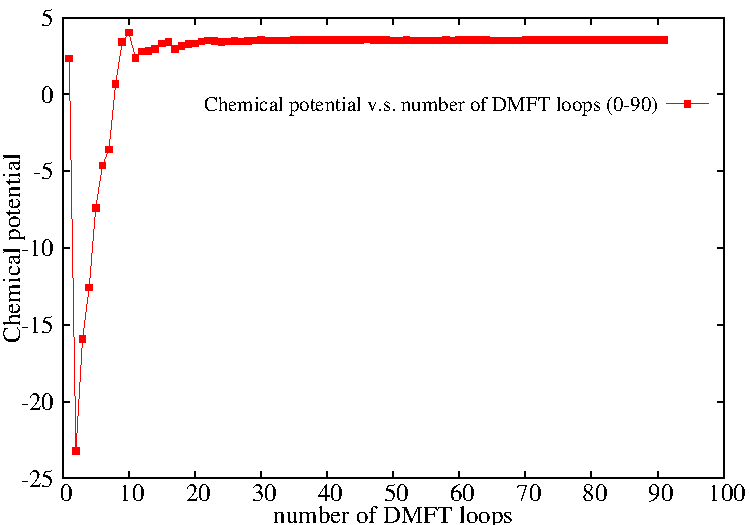
\includegraphics[scale=0.8]{gnuplotChemicalPotential1}
  \end{figure}

  Figure \ref{Chemical Potential v.s. number of DMFT loops in info.iterate 20 to 60} and Figure 
\ref{Chemical Potential v.s. number of DMFT loops in info.iterate 20 to 90} show the zoomed-in significant 
improvement feature of convergence by increasing the Monte Carlo number ``M'' from 12e6 (iteration 20-60) to 120e6 
(iteration 60-90). M number could be changed in \emph{params.dat} file. Also, you can keep M number the same, but
increase number of CPU cores by 10 times instead.  

  \cleardoublepage

  \begin{figure}[ht]
    \centering
    \captionsetup{justification=centering}
    \caption{Chemical Potential v.s. number of DMFT loops in \emph{info.iterate} 20 to 60}
    \label{Chemical Potential v.s. number of DMFT loops in info.iterate 20 to 60}
    \vspace{2ex}
    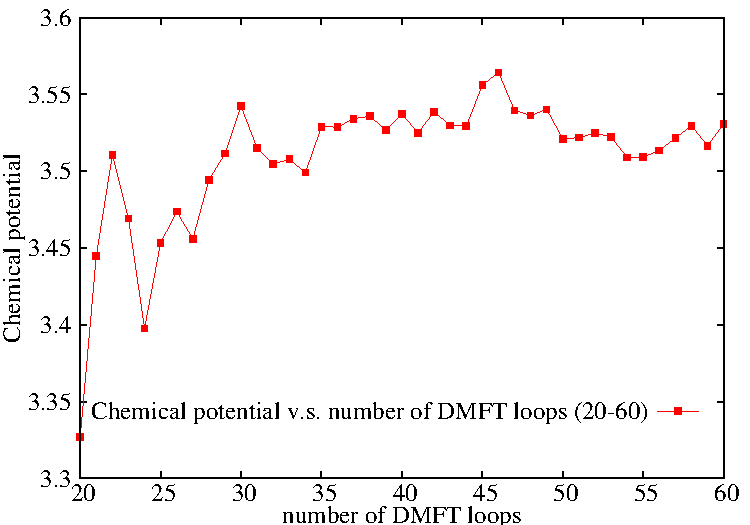
\includegraphics[scale=0.6]{gnuplotChemicalPotential2}
  \end{figure}

  \begin{figure}[ht]
    \centering
    \captionsetup{justification=centering}
    \caption{Chemical Potential v.s. number of DMFT loops in \emph{info.iterate} 20 to 90}
    \label{Chemical Potential v.s. number of DMFT loops in info.iterate 20 to 90}
    \vspace{2ex}
    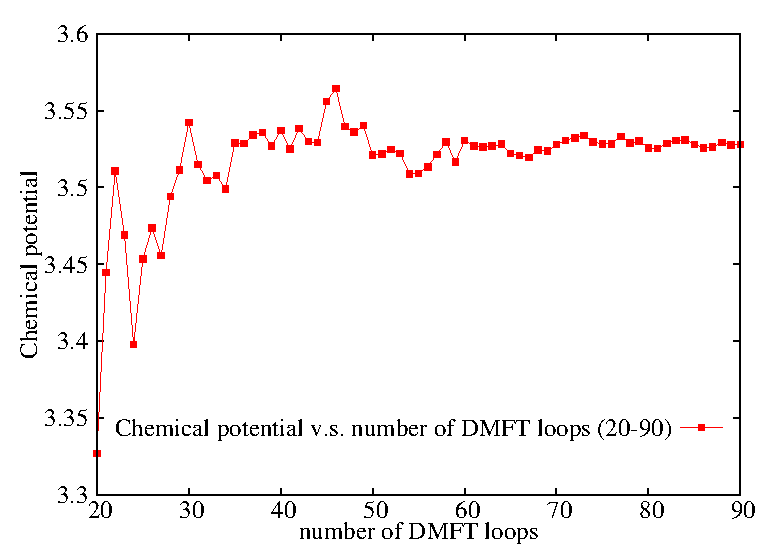
\includegraphics[scale=0.6]{gnuplotChemicalPotential3}
  \end{figure}

  \cleardoublepage

		  \item Plot impurity level v.s. number of DMFT loops in \emph{info.iterate} (see Figure 
\ref{Impurity level v.s. number of DMFT loops in info.iterate 0 to 90})

  \begin{figure}[ht]
    \centering
    \caption{Impurity level v.s. number of DMFT loops in \emph{info.iterate} 0 to 90}
    \label{Impurity level v.s. number of DMFT loops in info.iterate 0 to 90}
    \vspace{2ex}
    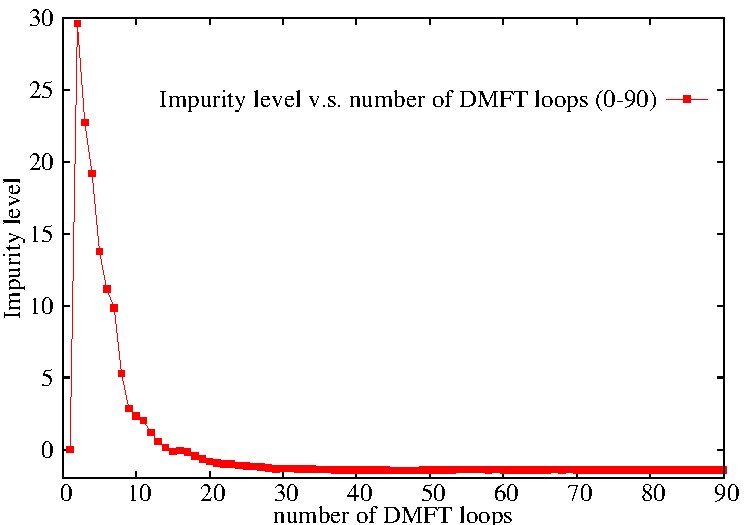
\includegraphics[scale=1.3]{gnuplotImpurityLevel}
  \end{figure}

  \cleardoublepage

		  \end{itemize}

	    \item Plot self-energies in \emph{sig.inp.*.1}

  We can check the convergence of DFT + DMFT iterations from self-energy files. Suppose we have finished 90 
iterations, then we plot the last 5 self-energy files, \emph{sig.inp.86.1, sig.inp.87.1, sig.inp.88.1, sig.inp.89.1 
sig.inp.90.1}. 

  The self-energies of $e_g$ orbitals in \emph{sig.inp.*.1} files are shown in Figure 
\ref{Self-energy v.s. number of DMFT loops in sig.inp.*.1 for eg orbitals}.

  The self-energies of $t_{2g}$ orbitals in \emph{sig.inp.*.1 files} are shown in Figure 
\ref{Self-energy v.s. number of DMFT loops in sig.inp.*.1 for t2g orbitals}.

  \begin{figure}[ht]
    \centering
    \caption{Self-energy v.s. number of DMFT loops in \emph{sig.inp.*.1} for $e_g$ orbitals}
    \label{Self-energy v.s. number of DMFT loops in sig.inp.*.1 for eg orbitals}
    \vspace{2ex}
    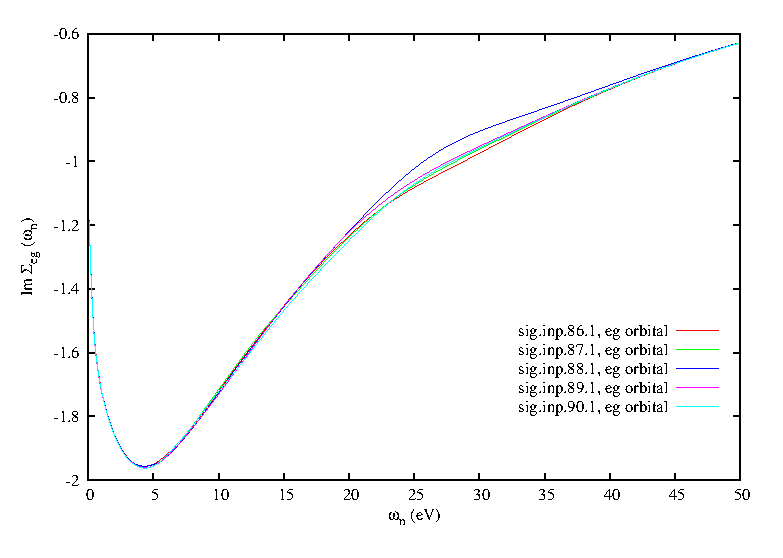
\includegraphics[scale=1.3]{gnuplotSelfEnergysiginpeg}
  \end{figure}

  \cleardoublepage

  \begin{figure}[ht]
    \centering
    \caption{Self-energy v.s. number of DMFT loops in \emph{sig.inp.*.1} for $t_{2g}$ orbitals}
    \label{Self-energy v.s. number of DMFT loops in sig.inp.*.1 for t2g orbitals}
    \vspace{2ex}
    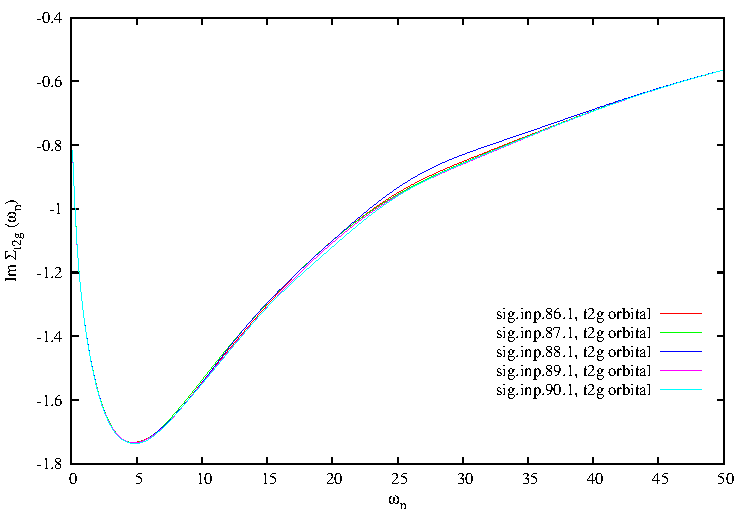
\includegraphics[scale=1.3]{gnuplotSelfEnergysiginpt2g}
  \end{figure}

	    \item Plot self-energies in \emph{sig.inp} and \emph{Sig.outb}

  Alternatively, you can check the quality of self-energy convergence by plotting the self-energy results in the 
following files, \emph{sig.inp} and \emph{imp.0/Sig.outb}. As can be seen, unconditioned self-energy pattern in 
\emph{Sig.outb} is quite scattered. There are two solutions to solve this problem, 1. Increase number of Monte 
Carlo cycle measurements by simply changing ``M'' value in the \emph{params.dat} file. 2. Increase number of CPU 
cores by modifying \emph{mpi} value in DMFT submit script.

  \cleardoublepage

		  \begin{itemize}[leftmargin=0.5in]

		  \item Plot conditioned self-energy in \emph{sig.inp} before and after augmenting Monte Carlo 
numbers

  Here illustrates conditioned self-energies before we increase the total Monte Carlo measurements (red line) 
and after the increase (green line) in \emph{sig.inp} (see Figure 
\ref{Conditioned self-energy v.s. number of DMFT loops in sig.inp before and after augmenting Monte Carlo
 measurements for eg orbitals})

  \begin{figure}[ht]
    \centering
    \captionsetup{justification=centering}
    \caption{Conditioned self-energy v.s. number of DMFT loops in \emph{sig.inp} before and after augmenting Monte 
Carlo measurements for $e_g$ orbitals}
    \label{Conditioned self-energy v.s. number of DMFT loops in sig.inp before and after augmenting Monte Carlo 
measurements for eg orbitals}
    \vspace{2ex}
    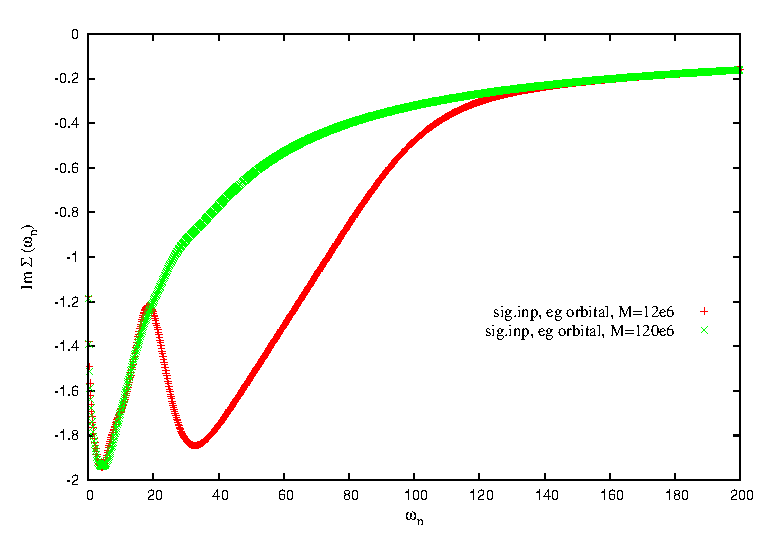
\includegraphics[scale=1.3]{gnuplotSelfEnergysiginpMC}   
  \end{figure}

  \cleardoublepage

		  \item Plot unconditioned self-energy in \emph{imp.0/Sig.outb} before and after augmenting Monte 
Carlo numbers

  Here shows unconditioned self-energies before we increase the total Monte Carlo measurements (red line) 
and after the increase (green line) in \emph{Sig.outb} (see Figure 
\ref{Unconditioned self-energy v.s. number of DMFT loops in Sig.outb before and after augmenting Monte Carlo 
measurements for eg orbitals}). It is obvious that the quality of unconditioned self-energy has been improved 
tremendously. 

  \begin{figure}[ht]
    \centering
    \captionsetup{justification=centering}
    \caption{Unconditioned self-energy v.s. number of DMFT loops in \emph{Sig.outb} before and after augmenting Monte
 Carlo measurements for $e_g$ orbitals}
    \label{Unconditioned self-energy v.s. number of DMFT loops in Sig.outb before and after augmenting Monte Carlo
 measurements for eg orbitals}
    \vspace{2ex}
    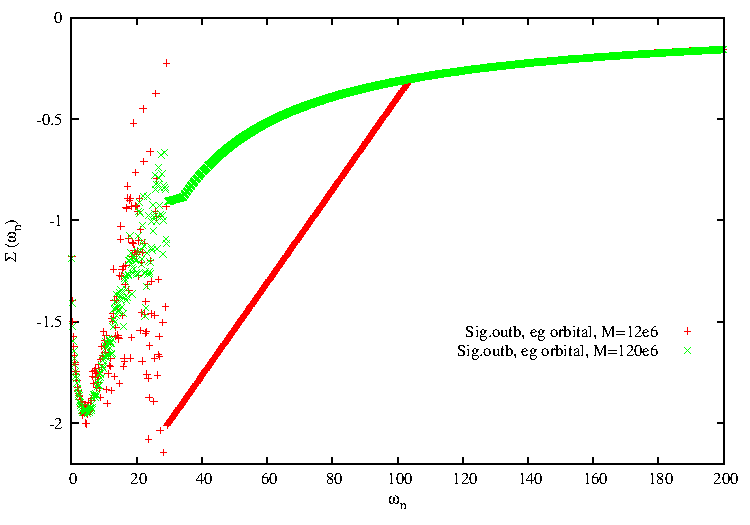
\includegraphics[scale=1.3]{gnuplotSelfEnergySigoutbMC}
  \end{figure}

  \cleardoublepage

		  \item Conditioning of self-energy in \emph{Sig.out}

  In DFT + DMFT, only the first ``nom'' Matsubara frequency points are directly from Quantum Monte Carlo (QMC) 
outputs using the Dysons' calculated equations. 

  $\Sigma(i\omega n)$ = $G^{o -1}(i\omega n)$ - $G^{-1}(i\omega n)$

  Green's function has a $\frac{1}{×i\omega n}$ asymptotic behavior and at the high frequency/energy region, 
$G(i\omega n)$ and $G^o(i\omega n)$ will be close to zero value. Due to the systematic error in QMC measurements, 
$\Sigma(i\omega n)$ at high frequency will have a very large scattering, as can be seen in \emph{imp.0/Sig.outb} at 
frequencies near $\omega_n = 65$. 
(see Figure \ref{Imaginary part of self-energy v.s. real frequency in Sig.out for eg and t2g orbitals}). 

  \begin{figure}[ht]
    \centering
    \captionsetup{justification=centering}
    \caption{Imaginary part of self-energy v.s. real frequency in Sig.out for $e_g$and $t_{2g}$ orbitals}
    \label{Imaginary part of self-energy v.s. real frequency in Sig.out for eg and t2g orbitals}
    \vspace{2ex}
    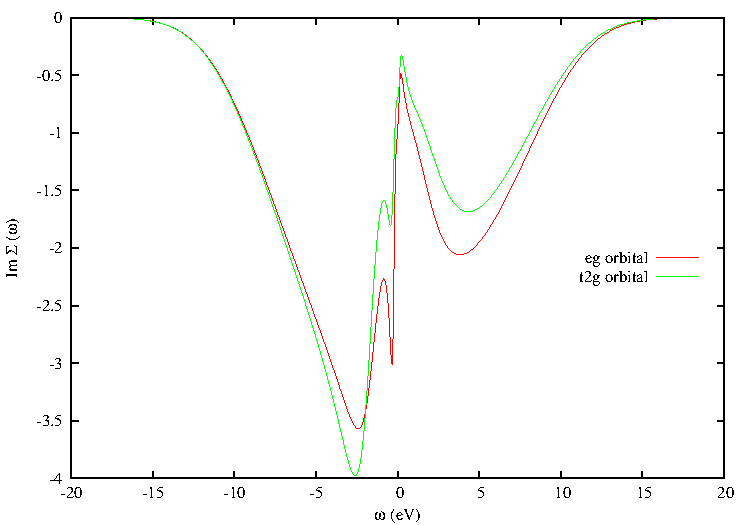
\includegraphics[scale=1.3]{gnuplotImaginaryPartRealFrequency}
  \end{figure}

  Since we know the high frequency asymptotic behavior of self-energy, then the high frequency tail of self-energy at 
number of $\omega_n >$ ``nom'' is given by the high frequency asymptotic functional; and the self-energy points 
from [non-nom, nom] is used to fix the parameters of asymptotic functional. 

		  \end{itemize} 

	      \end{itemize}

%  \hyperlink{my toc}{Back to Table of Contents}
  
  \cleardoublepage

  \part{Test cases}

    \section{FCC Fe at 1500 K 0 GPa}

  First, we want to test the DFT + DMFT calculations on a simple test case, FCC Fe at 1500 K 0 GPa, which has 
1 atom per primitive cell and paramagnetic. 

      \subsection{Run DFT+DMFT codes}

	\subsubsection{Prepare struct-files}

	  \begin{itemize}[leftmargin=0.2in]

	    \item Gather all the required information

	    \begin{itemize}

	      \item The lattice parameters,

  lengths a, b, c in Bohr or \AA{ngstrom} and angles $\alpha$, $\beta$, $\gamma$.

	      \item The space group according to the ``International Tables for Crystallography'', 
  
  \url{http://it.iucr.org/}

	      \item The positions of all inequivalent atoms in fractions of the unit cell. 

	    \end{itemize}

  \cleardoublepage

	    \item Manually set up the struct-files

  Create a new \emph{.txt} file by the command 

  ``\textbf{vi FCC\_Fe}'' 

  in your new folder \emph{FCC\_Fe}. Next, type in all the prepared lattice information, (see Table 
\ref{Lattice parameters in FCC_Fe text file})

  \begin{table}[ht]
    \centering
    \caption{Lattice parameters in \emph{FCC\_Fe} text file}
    \label{Lattice parameters in FCC_Fe text file}
    \vspace{2ex}
  \begin{tabular}{|l|l|l|l|l|l|l|}

  \hline
  \textbf{b}		&			&			&	&	& 		& ``a..Ang, 
b..Bohr''\\ \hline

  \textbf{0.0} 		& \textbf{0.0} 		& \textbf{0.0}		&	&	& 		& ``shift of 
origin''\\ \hline

  \textbf{8.1450} 	& \textbf{8.1450} 	& \textbf{8.1450} 	& \textbf{90} 	& \textbf{90} 	& \textbf{90}
	& ``a, b, c, angles $\alpha, \beta, \gamma$''\\ \hline

  \textbf{Fm-3m}	&			&			&	&	&		& 
``space-group symbol''\\ \hline

  \textbf{Fe}		&			&			&	&	&		& ``atom-
name''\\ \hline

  \textbf{0.0000000} 	& \textbf{0.0000000} 	& \textbf{0.0000000}	&	&	&		& ``atomic
 position''\\ \hline

  \end{tabular}
  \end{table}

  Exit editing and save the text file, then the \emph{FCC\_Fe} text file has been made. Next task is to create your 
struct-file, \emph{FCC\_Fe.struct}, by the command 

  ``\textbf{cif2struct FCC\_Fe}''

  in your current directory. You can further modify the title and the automatically calculated values in the 
established struct-file.

  \cleardoublepage

	  \end{itemize}

	\subsubsection{Initialize calculations using init\_lapw}

  \emph{FCC\_Fe.struct} file contains all the information needed for the crystal structure calculations that 
WIEN2k uses. Run the following command, 

  ``\textbf{init\_lapw}''

  The following shows all the subsequent questions and corresponding default answers.

  \begin{enumerate}

   \item The screen first shows:

  next is setrmt. 

  Automatic determination of RMTs. Please specify the desired RMT reduction compared to almost touching spheres.

  Typically, for a single calculation just hit enter, for force minimization use 1-5; for volume effects you may 
need even larger reductions. 

  Press ``\textbf{Enter}''

   \item You will choose answers to a series of questions, typically you will enter the default setting values 
that WIEN2k uses as follows,

  ``\textbf{o, a, 2, c, c, c, -up, 13, -6, c, 200, c, n}''

  which stands for the following meanings respectively:

  \emph{o}: use old scheme; 

  \emph{a}: accept these radii; 

  \emph{2}: nn-bondlength factor;

  \emph{c}: continue with sgroup; 

  \emph{c}: continue with symmetry; 

  \emph{c}: continue with lstart; 

  \emph{-up}: switches for instgen\_lapw -up(default); 

  \emph{13}: SELECT XCPOT, 13:PBE-GGA (Perdew\_Burke-Ernzerhof 96); 

  \emph{-6}: SELECT ENERGY to separate core and valence states: -6.0 Ry (check how much core charge leaks out of
 MT-sphere); 

  \emph{c}: continue with kgen; 

  \emph{200}: number of k-points in whole cell, usually 200-500; 

  \emph{c}: continue with dstart; 

  \emph{n}: not perform a spinpolarized calculation. 

  \end{enumerate}

  \cleardoublepage

	\subsubsection{Run the self-consistency cycles (SCF) of DFT calculations}

  After \emph{init\_lapw}, there are many new files generated in the \emph{FCC\_Fe} folder. The next step is 
to run self-consistency cycles (SCF) of DFT calculations. It is strongly suggested to submit the DFT calculations 
job via the \emph{submit\_dft.scr} script utilizing services provided by a parallel computing machine 
(e.g., \emph{mw} server). An example of \emph{submit\_dft.scr} is shown in the Part III. The command to submit the 
DMFT calculation job to \emph{mw} server is as follows,

  ``\textbf{qsub submit\_dft.scr}''
 
  Another way to run SCF is to use the command ``\textbf{run\_lapw}'', but it is not recommended.

  The self-consistency cycles (SCF) consist of the following parts:

  \emph{LAPW0} (POTENTIAL) generates potential from density

  \emph{LAPW1} (BANDS) calculates valence bands (eigenvalues and eigenvectors)

  \emph{LAPW2} (RHO) computes valence densities from eigenvectors

  \emph{LCORE} computes core states and densities

  \emph{MIXER} mixes input and output densities

  After SCF of DFT calculations, good charge densities have been converged. You can save your results by the 
command ``\textbf{save\_lapw}''.   

  \cleardoublepage

	\subsubsection{Initialize DMFT calculations}

  Following \emph{init\_lapw} and SCF of DFT, proceed to the command 

  ``\textbf{init\_dmft.py}''

  to invoke DMFT calculations in the current directory. 

  Suggestions on the choices thereafter are shown below, 

  \begin{itemize}

    \item Specify correlated atoms (e.g. 1-4, 7, 8): \textbf{1}

    \item Type ``\textbf{c}''

    \item For each atom, specify correlated orbital(s) (e.g. d, f): \textbf{d}

    \item Type ``\textbf{c}''

    \item Specify qsplit for each correlated orbital (default = 0): \textbf{7} (cubic symmetry in real harmonics) 

    \item Type ``\textbf{c}''

    \item Do you want to group any of these orbitals into cluster-DMFT problems? (y/n): \textbf{n}

    \item Enter the correlated problems forming each unique correlated problem, separated by spaces (e.g. 
1, 3 2, 4 5-8) \textbf{1}

    \item Type ``\textbf{c}''

    \item Broken symmetry run? (y/n): \textbf{n}

    \item Range (in eV) of hybridization taken into account in impurity problems; default -6.0, 6.0: -10, 10: 
\textbf{-10, 10}

    \item Perform calculations on real; or imaginary axis? (r/i): \textbf{i}

    \item Is this a spin-orbit run? (y/n): \textbf{n}

    \item Generate blank sig.inp? (y/n): \textbf{y}

  \end{itemize}
  
  \cleardoublepage

	\subsubsection{Prepare all files}

	\begin{itemize}[leftmargin=0.2in]

	  \item Prepare input files (\emph{FCC\_Fe.indmfl}, \emph{FCC\_Fe.indmfi}) and output files

  The initialization of DMFT calculations by \emph{init\_dmft.py} will generate two input files, \emph{FCC\_Fe.indmfi} 
and \emph{FCC\_Fe.indmfl}. These two files will connect the solid and impurity with DMFT equations. 

  Create a new folder that is in the parent directory, 

  ``\textbf{mkdir FCC\_Fe\_backup}''

  then move all the files from \emph{FCC\_Fe} folder into the \emph{FCC\_Fe\_backup} folder by the command,

  ``\textbf{mv ./* ../FCC\_Fe\_backup/}''

  then type in the following command in the current directory (\emph{FCC\_Fe}/),

  ``\textbf{dmft\_copy.py $<$parent directory$>$/FCC\_Fe\_backup/ -a}''

  -a: files for both DFT and DMFT will be copied. 

  This command makes a copy of all the output files of DFT calculation results and DMFT initialization results 
into the folder \emph{FCC\_Fe}. These files are needed for the following DMFT calculations. Examples of copied 
files are listed below,

  struct-file, WIEN2k files (\emph{.in0, .in1, .in2, .inm, .inso, .inc)}, charge density file (\emph{.clmsum}), 
input files (\emph{.indmfi, .indmfl}) and other files (\emph{.klist, .kgen, .scf2})

	  \item Prepare \emph{params.dat} and \emph{sig.inp} files

  We need to prepare two more files needed for DMFT calculations in the \emph{FCC\_Fe} folder, \emph{params.dat} 
and \emph{sig.inp}. 

	    \begin{itemize}

	    \item \emph{params.dat}

  Manually set up the \emph{params.dat} file or download the \emph{params.dat} file from Haule's W2K Database website, 

  \url{http://hauleweb.rutgers.edu/database_w2k/}

  The \emph{params.dat} file contains information about the program flow and impurity solver. Leave the 
\emph{params.dat} file name as it is. In the \emph{params.dat} file, you can change the following parameters,

	      \begin{itemize}

	      \item finish=

  The number of charge self-consistent iterations in \emph{params.dat} file, e.g., \textbf{finish=60} means there are
 60 iterations in DFT+DMFT calculations. 

	      \item iparams0=\{``beta''\}

  ``beta'' is the inverse temperature. It is derived from the absolute temperature in Kelvin, $\beta=\frac{1(eV)}
{×T(K)}$ in which $1eV=11604K$. For example, if absolute temperature T is 300 K, then $\beta=\frac{11604K}{×300K}=
38.68$. \textbf{``beta'': 38.68}.

	      \item iparams0=\{``M''\}

  ``M'' is the Total number of Monte Carlo steps. Typical \emph{M} is 5 million (5e6), i.e., \textbf{``M'': 5e6}. 
Total Monte Carlo measurements (N) is calculated by the equation, \emph{N = (Number of CPU) * M}. (\emph{Number of 
CPU}) could be changed in \emph{mpi} value in the \emph{submit\_dmft.scr} file.

	      \end{itemize}

  \cleardoublepage

	    \item \emph{sig.inp}

  \emph{sig.inp} is a blank self-energy file, it is generated by the command 

  ``\textbf{szero.py -e 35.7 -T 0.026 -n 3000}''

  Make sure that the \emph{T} value here (0.026) is the same as the \emph{beta} value in \emph{params.dat} file. The 
meanings of the characters (\emph{e, T, n}) are as follows,

	      \begin{itemize}

	      \item e

  Double counting energy, calculated by the equation

  $E_{DC}$=U(n-$\frac{1}{×2}$)-J/2(n-1) 

  in which $U=6\ eV$; $J=0.8\ eV$

	      \item T

  Effective temperature in DMFT which should be consistent with \emph{beta} in the \emph{params.dat} file. For 
example, if we have \emph{beta=38.68333}, then $T=\frac{1}{×beta}=\frac{1}{×38.68333}=0.026$. Please notice that 
\emph{T} here is the effective temperature in DMFT derived from \emph{beta} which is different from the absolute 
temperature. 

	      \item n

  The number of Matsubara frequency points

	      \end{itemize}

	  \end{itemize}

	\end{itemize}

	\subsubsection{Submit the job and run DFT + DMFT iterations}

  Copy \emph{submit\_dmft.scr} script file into the current directory (\emph{FCC\_Fe}). An example of 
\emph{submit\_dmft.scr} file is shown in Part III. The final step is to type in the command,

  ``\textbf{qsub submit\_dmft.scr}''

  Using the remote powerful machine (mw) is handy in terms of computing a large number of Monte Carlo cycles due to a 
large number of CPU cores it has. The command above is going to create a \emph{.dat} file for mpi parallel execution, 
\emph{mpi\_prefix.dat}. 

  \cleardoublepage

	\subsubsection{Monitor running of DFT + DMFT}

  During the run, we can monitor the information file and update parameters, if necessary. The files we can monitor
 are listed below,

	\begin{itemize}

	 \item \emph{info.iterate}

  It contains information about chemical potential, impurity levels, exchange energies and total fillings, etc. 

	\item \emph{:log}

  It helps monitor the modules that are running.

	\item \emph{dmft\_info.out, FCC\_Fe.dayfile}

  To monitor the DMFT calculations and convergence levels.

	\item \emph{imp.0/nohup\_imp.out, imp.0/Sig.out, imp.0/Gf.out}

  To monitor the impurity levels. 

	\item \emph{dmft1\_info.out, FCC\_Fe.outputdmf1.0}

  To monitor the dmft1 step. 

	\item \emph{dmft2\_info.out, FCC\_Fe.outputdmf2.0}

  To monitor the dmft2 step.

	\end{itemize}

%  \hyperlink{my toc}{Back to Table of Contents}
  
  \cleardoublepage

      \subsection{Properties based on DMFT calculations}

  Once the SCF cycle has converged one can calculate various properties, such as Probabilities, Density of States 
(DOS), Partial Density of States (Partial DOS), spectral functions, optics (including conductivity) and Fermi surface.

  Let's continue with our simplest test case, \emph{FCC Fe at 1500 K 0 GPa}, and calculate properties based on it.

	\subsubsection{\emph{histogram.dat} and \emph{Probability.dat}}

  \begin{itemize}

   \item \emph{histogram.dat}

  To check whether the parameter ``Nmax'' in the \emph{params.dat} file is large enough, we should plot 
``imp.0/histogram.dat'', which should be gaussian, and should look like figure \ref{Plot histogram.dat file}.

  \begin{figure}[h]
    \centering
    \captionsetup{justification=centering}
    \caption{Plot \emph{histogram.dat} file}
    \label{Plot histogram.dat file}
    \vspace{2ex}
    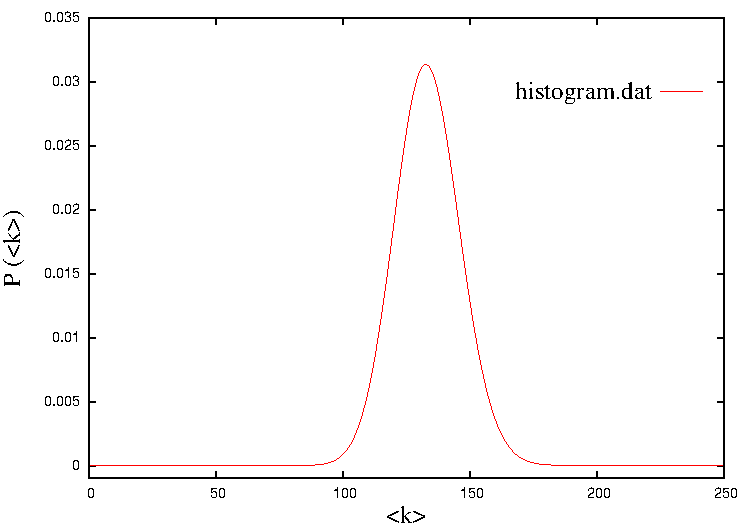
\includegraphics[scale=0.8]{gnuplothistogram}
  \end{figure}

  This shows the distribution of the perturbation order. The perturbation order around 200 has almost no probability, 
hence Nmax=400 (two kinks for each perturbation order) would be sufficient. We used substantially larger Nmax=600, 
so that we could reduce the temperature for factor of 3. Notice that larger Nmax only slightly slows down the execution 
of the code, and uses only a bit more memory, hence it is a good idea to use large Nmax.

   \item \emph{imp.0/Probability.dat}

  We can also check what the probability for each atomic state is, i.e., probability that a Fe-d electron is in any 
of the atomic states. This information is written in ``imp.0/Probability.dat''. The first and the second column 
correspond to the index of each spin configuration, as defined in ``actqmc.cix'' (which enumerates all atomic states).
 The third column is the probability for a state. Here is the plot of probability for first 170 states, see figure 
\ref{Plot imp.0/Probability.dat file 0-170},
  
  \begin{figure}[ht]
    \centering
    \captionsetup{justification=centering}
    \caption{Plot \emph{imp.0/Probability.dat} file}
    \label{Plot imp.0/Probability.dat file 0-170}
    \vspace{2ex}
    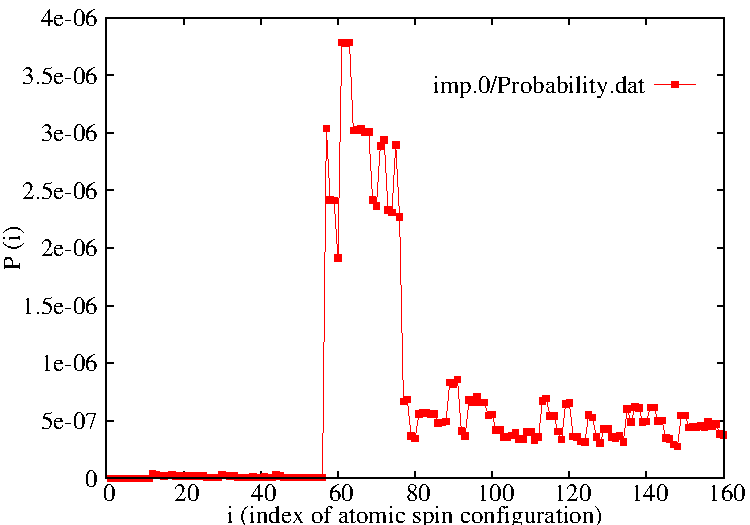
\includegraphics[scale=0.8]{gnuplotProbability}
  \end{figure}

  The first state corresponds to the empty 4f ion. The next 80 states (from 1...80) correspond to nominal occupancy 
N=1, and the values between 80 and 170 correspond to occupancy N=2. At N=1, there are two sets of probabilities, 6 
take the value around 4e-6, and 8 take the value of 2e-6. The first and the second set corresponds to j=5/2 and 
j=7/2 multiplet, respectively. The next 90 states, which correspond to occupancy N=2, have probability around 5e-7. 
They can be grouped into multiplets, the lowest being J=4, followed by J=2 and J=5. Notice that the lowest multiplet 
satisfies Hunds rules (largest S=1, largest L=5, and J=L-S=4). Notice also that although FCC Fe is a very itinerant 
metal, the projection to the atomic states still satisfies atomic rules, such as Hunds rules. The cumulative 
probability for N=2 states is around 0.086. Compare this to N=1 probability of 0.836, and N=0 probability of 0.077. 
The next 430 states correspond to N=3 occupancy, and their histogram looks like figure 
\ref{Plot imp.0/Probability.dat file 0-600}.
  
  \begin{figure}[ht]
    \centering
    \captionsetup{justification=centering}
    \caption{Plot \emph{imp.0/Probability.dat} file 0-600}
    \label{Plot imp.0/Probability.dat file 0-600}
    \vspace{2ex}
    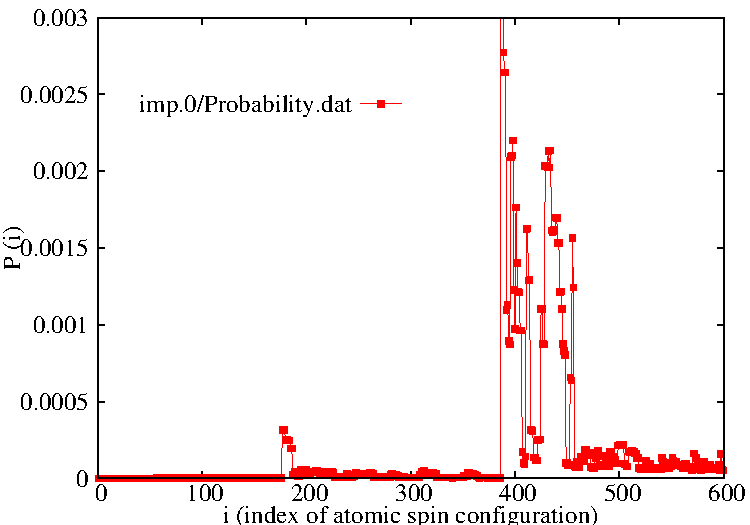
\includegraphics[scale=0.8]{gnuplotProbability2}
  \end{figure}

  Typical probability of N=3 state is 1e-6, and cumulative probability is 0.0012. Clearly, the probability falls off 
very rapidly with particle number N, hence we can safely restrict occupancy in params.dat file to nc=[0, 1, 2, 3].

  \end{itemize}

  \cleardoublepage

	\subsubsection{\texorpdfstring{Density of States (DOS) and Partial Density of States\\ (Partial DOS)}{Density 
of States (DOS) and Partial Density of States(Partial DOS)}} 

	  \begin{itemize}[leftmargin=0in]

	  \item Analytical continuation of self energies

  We are going to do analytical continuation to calculate the self energy on the real axis after acquiring our results 
on the imaginary axis.

  \vspace{10ex}

  \begin{picture}(,)
  \centering
   
    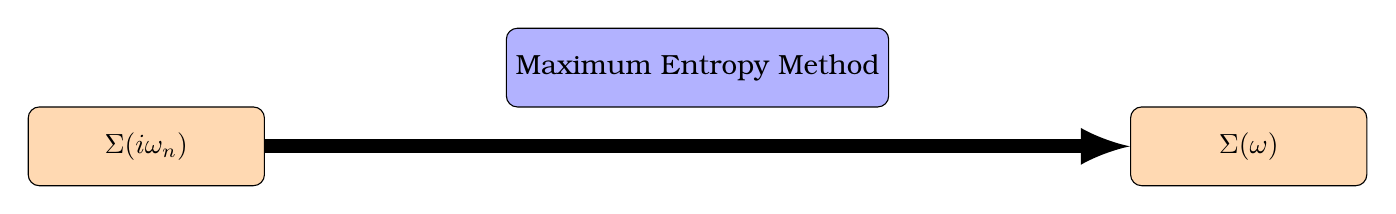
\begin{tikzpicture}[node distance=1cm]
     
  \node(anchor)[DFT]{Maximum Entropy Method};
  \node(imaginary)[DMFT, below of=anchor, xshift=-7cm]{$\Sigma(i\omega_n)$};
  \node(real)[DMFT, below of=anchor, xshift=7cm]{$\Sigma(\omega)$}
    edge[arrow, <-](imaginary);

    \end{tikzpicture}

  \end{picture}


  \begin{enumerate}

  \item Preparation: make several new directories under the parent directory 

(\emph{FCC\_Fe}) before we do any calculations on DOS, \textbf{DOS/FCC\_Fe, mem/Sig\_real} and \textbf{mem/Gf\_real}

  \item Average the self-energies from the last few iterations to minimize the noise, 

  \textbf{saverage.py sig.inp.86.1 sig.inp.87.1 sig.inp.88.1 sig.inp.89.1\\ sig.inp.90.1 sig.inpx}

  Here it averages the last five \emph{sig.inp.*.1} files and creates an output file \emph{sig.inpx} in the current 
directory \emph{FCC\_Fe}.

  \item Copy the averaged self energy file \emph{sig.inpx} into the new folder \emph{mem/Sig\_real}. 

  \item Download and modify \emph{maxent\_params.dat} file from Haule's website, 
\url{http://hauleweb.rutgers.edu/downloads/}. 

  Make sure 'Ntau' value in \emph{maxent\_params.dat} file matches \emph{beta} value in\\ \emph{params.dat} file. Copy 
modified \emph{maxent\_params.dat} file into the same directory \emph{mem/Sig\_real}. This file contains the 
parameters needed for analytical continuation process.

  \item Run the maximum entropy method (mem). 

  Now there are two files in \emph{mem/Sig\_real} folder, \emph{sig.inpx}\\ and \emph{maxent\_params.dat}. Next 
execute the command,

  \textbf{maxent\_run.py sig.inpx}

  to produce the self energy file \emph{Sig.out} on the real axis. Results in 
\emph{Sig.out} file are plotted in Figure 
\ref{Imaginary part of self-energy v.s. real frequency in Sig.out for eg and t2g orbitals}, 
\ref{Real part of self-energy v.s. real frequency in Sig.out for eg and t2g orbitals}.
  
  \end{enumerate}

  \vspace{10ex}

  \begin{picture}(,)
  \centering
   
    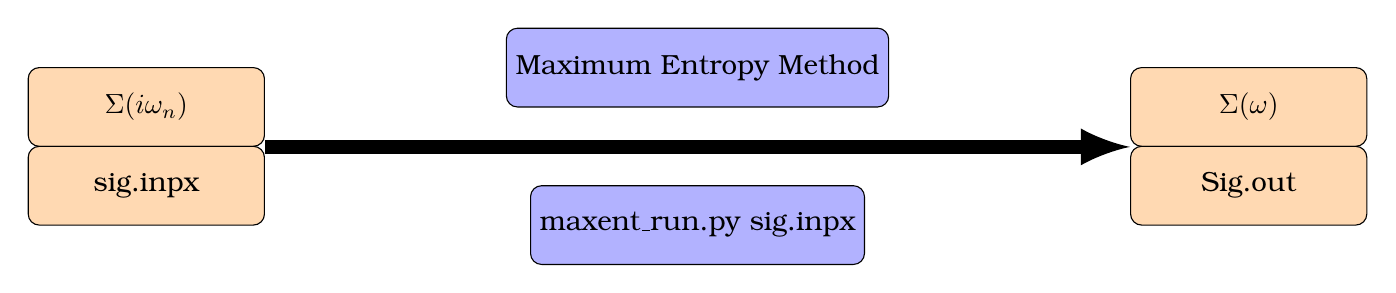
\begin{tikzpicture}[node distance=0.5cm]
     
  \node(anchor)[DFT]{Maximum Entropy Method};
  \node(imaginary)[DMFT, below of=anchor, xshift=-7cm]{$\Sigma(i\omega_n)$};
  \node(real)[DMFT, below of=anchor, xshift=7cm]{$\Sigma(\omega)$};
%     edge[arrow, <-](imaginary);
  \node(anchor2)[DFT, below of=anchor, yshift=-1.5cm]{maxent\_run.py sig.inpx};
  \node(siginp)[DMFT, below of=imaginary, yshift=-0.5cm]{sig.inpx};
  \node(Sigout)[DMFT, below of=real, yshift=-0.5cm]{Sig.out};
  \path (imaginary.south east) edge[arrow] (real.south west);

    \end{tikzpicture}

  \end{picture}

  \begin{figure}[ht]
    \centering
    \captionsetup{justification=centering}
    \caption{Real part of self-energy v.s. real frequency in Sig.out for $e_g$and $t_{2g}$ orbitals}
    \label{Real part of self-energy v.s. real frequency in Sig.out for eg and t2g orbitals}
    \vspace{2ex}
    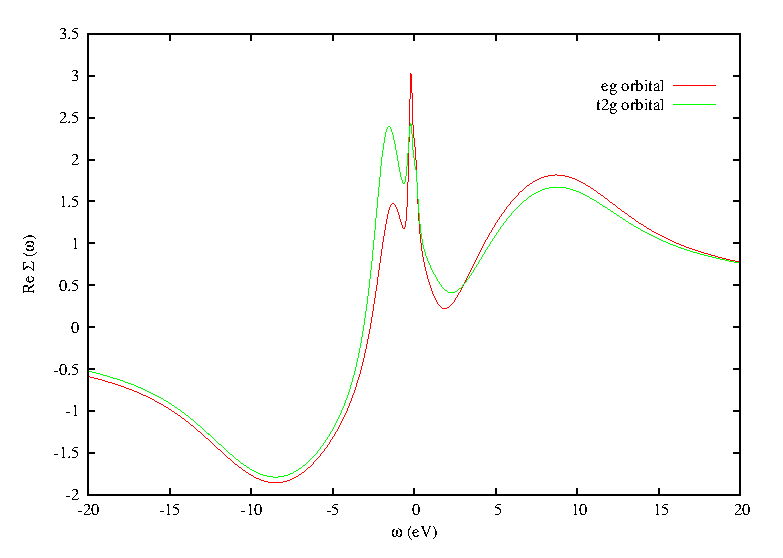
\includegraphics[scale=1.3]{gnuplotRealPartRealFrequency}
  \end{figure}
  
  \cleardoublepage

	      \item Plot Total DOS

  To plot Total Density of States (DOS), we need to run one more dmft1 calculation to obtain Green's function and DOS 
on the real axis. 

  \begin{enumerate}[leftmargin=0.2in]

    \item Now we are going to work in the directory \emph{/FCC\_Fe/DOS/FCC\_Fe/}, first, copy all the DMFT output 
files,

  \textbf{dmft\_copy.py ../../ -a}

    \item Copy the generated \emph{Sig.out} file to \emph{sig.inp} in current directory (/DOS/FCC\_Fe/)

  \textbf{cp ../../mem/Sig\_real/Sig.out sig.inp}

    \item Modify \emph{FCC\_Fe.indmfl} file by changing 'Matsubara' value on the second line from imaginary axis 
``\textbf{1}'' to real axis ``\textbf{0}''.

    \item Run \textbf{x kgen} and specify number of k-points in whole cell, \textbf{8000}

    \item Run dmft1 calculations once,

  \textbf{x lapw0}

  \textbf{x lapw1}

  \textbf{x\_dmft.py dmft1}

    \item Plot the Total Density of States (DOS) which is stored in the \emph{FCC\_Fe.cdos} file. Results of Total 
DOS are shown in Figure \ref{Total Density of States on the real axis for FCC Fe}.

  \end{enumerate}

  \begin{figure}[ht]
    \centering
    \caption{Total Density of States on the real axis for FCC Fe}
    \label{Total Density of States on the real axis for FCC Fe}
    \vspace{2ex}
    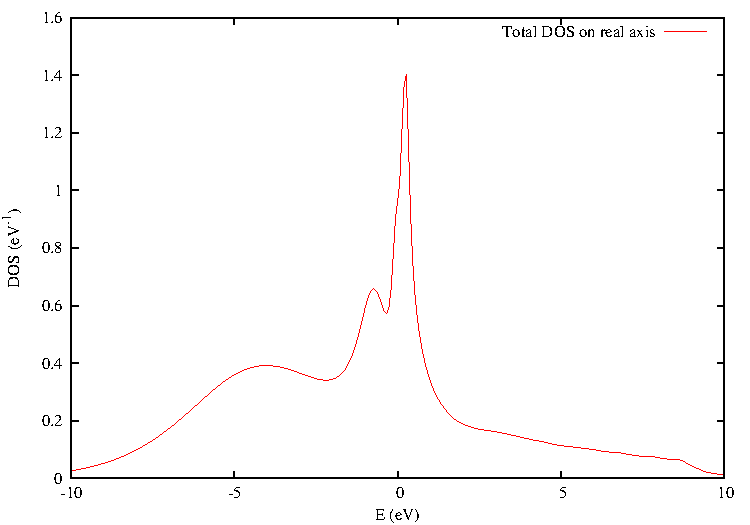
\includegraphics[scale=1.3]{gnuplotTotalDOS}
  \end{figure}

  \cleardoublepage

	      \item Plot Partial DOS

  Now we move on to calculate and plot the partial (d-orbital) Density of States (DOS).

  \begin{itemize}[leftmargin=0.2in]

    \item We are going to work in the new directory \emph{FCC\_Fe/mem/Gf\_real}

    \item Copy \emph{maxent\_params.dat} and \emph{Gf.out} files into \emph{Gf\_real} directory from directories, 
\emph{/FCC\_Fe/mem/Sig\_real/maxent\_params.dat} and \emph{/FCC\_Fe/imp.0/Gf.out} respectively.

    \item Run \textbf{maxent\_S.py Gf.out} in the current \emph{mem/Gf\_real} directory.

    \item Plot 'Sig.out' file generated. Note that partial DOS is given by dividing the imaginary part of the Green's 
function by $-\pi$.

  $A(\omega) = -1/\pi*(Im G(\omega))$

  So the commands should resemble the following,

  \textbf{plot 'Sig.out' u 1:(-\$3/3.14) w l} ``:DOS of $e_g$ d orbital''

  \textbf{plot 'Sig.out' u 1:(-\$5/3.14) w l} ``:DOS of $t_{2g}$ d orbital''

    \item The results of all partial d orbital DOS are shown in Figure 
\ref{Partial Density of States (eg and t2g) on the real axis for FCC Fe}. The comparison between the partial DOS and 
total DOS is shown in Figure \ref{Partial Density of States and Total Density of States on the real axis for FCC Fe}.

  \end{itemize}
	  
	      \end{itemize}

  \cleardoublepage

  \begin{figure}[ht]
    \centering
    \caption{Partial Density of States ($e_g$ and $t_{2g}$) on the real axis for FCC Fe}
    \label{Partial Density of States (eg and t2g) on the real axis for FCC Fe}
    \vspace{2ex}
    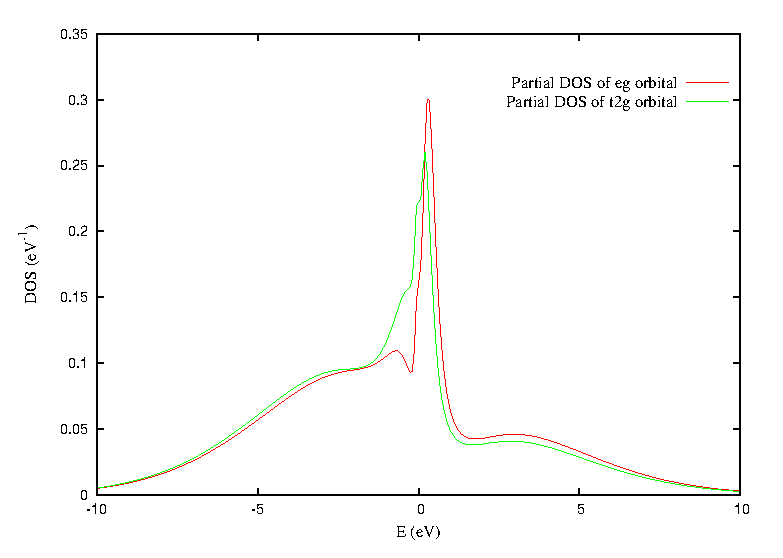
\includegraphics[scale=1.3]{gnuplotPartialDOS}
  \end{figure}

  \begin{figure}[ht]
    \centering
    \captionsetup{justification=centering}
    \caption{Partial Density of States and Total Density of States on the real axis for FCC Fe}
    \label{Partial Density of States and Total Density of States on the real axis for FCC Fe}
    \vspace{2ex}
    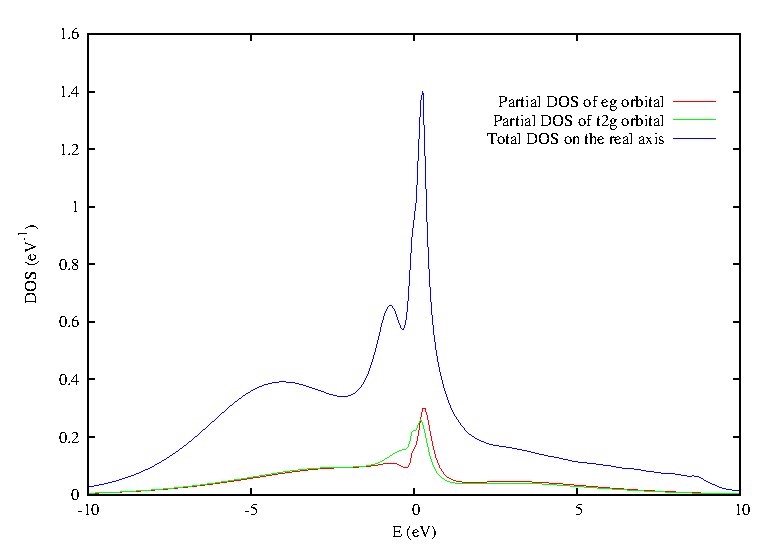
\includegraphics[scale=1.3]{gnuplotPartialDOSTotalDOS}
  \end{figure}

  \cleardoublepage

      \subsubsection{Spectral functions}

  \begin{enumerate}

    \item Preparation: Make a new folder containing all the results of calculations on Spectral functions (momentum 
resolved spectral function, equivalent to band structures in DFT). 

  \textbf{mkdir -p /FCC\_Fe/spectra/FCC\_Fe}

    \item Copy all the required files from DMFT calculations to the current directory. 

  \textbf{dmft\_copy.py ../../ -a}

  Here make sure you have \emph{EF.dat} file, if you don't, find the Fermi Energy and store the Fermi Energy to 
\emph{EF.dat} file in eV.

    \item Replace the imaginary self-energy by self-energy in real frequency. 

  \textbf{cp /FCC\_Fe/mem/Sig\_real/Sig.out sig.inp}

    \item Edit \emph{FCC\_Fe.indmfl} file. 

  On the second line of \emph{FCC\_Fe.indmfl} file, you will see,

{\color{cyan}

  1 0.025 0.025	600	-3.0000000	1.0000000	\# matsubara, broadening-corr, broadening-noncorr, nomega, 
omega\_min, omega\_max (in eV)

}

  Change the ``\emph{matsubara}'' value from \textbf{1} to \textbf{0} in order to switch from imaginary axis to real 
axis. Change the frequency range: ``\emph{omega\_min}'' from \textbf{-3} to \textbf{-5}; ``\emph{omega\_max}'' from 
\textbf{1} to \textbf{5}.

    \item Create \emph{FCC\_Fe.klist\_band} file to choose the path in momentum space (first brillouin zone).

  Figure \ref{First Brillouin Zone of FCC Fe lattice} illustrates the first Brillouin zone of a face centered cubic 
lattice, e.g. FCC Fe. 

  There are two ways to create this file. One is to write it by hand. The other method is to make a copy from WIEN2k 
prepared templates. Because FCC iron is the current system, we can simply copy \emph{fcc.klist} from WIEN2k templates. 

  \textbf{cp \$WIENROOT/SRC\_templates/fcc.klist FCC\_Fe.klist\_band}

    \item Run the following commands to execute DMFT calculations on the mesh in the current \emph{/spectra/FCC\_Fe/}
 directory.

  \textbf{x lapw0}

  \textbf{x lapw1 -band}

  \textbf{ssplit.py -i sig.inp}

  \textbf{x\_dmft.py dmftp}

    \item Plot the band structures by,

  \textbf{wakplot.py}

  You can increase the intensity of brightness by reducing it from 0.2 (default) to any smaller number. Here shows 
how the plot looks like (see Figure \ref{Spectral functions of FCC Fe}),
 
  \end{enumerate}

  \cleardoublepage

  \begin{figure}[ht]
    \centering
    \caption{First Brillouin Zone of FCC Fe lattice}
    \label{First Brillouin Zone of FCC Fe lattice}
    \vspace{2ex}
    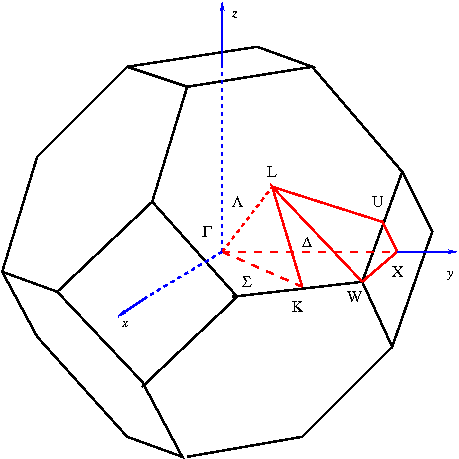
\includegraphics[scale=0.43]{FCC_Fe_brillouin}
  \end{figure}

  Source: \url{http://commons.wikimedia.org/wiki/File:Fcc_brillouin.png}


  \begin{figure}[ht]
    \centering
    \caption{Spectral functions of FCC Fe}
    \label{Spectral functions of FCC Fe}
    \vspace{2ex}
    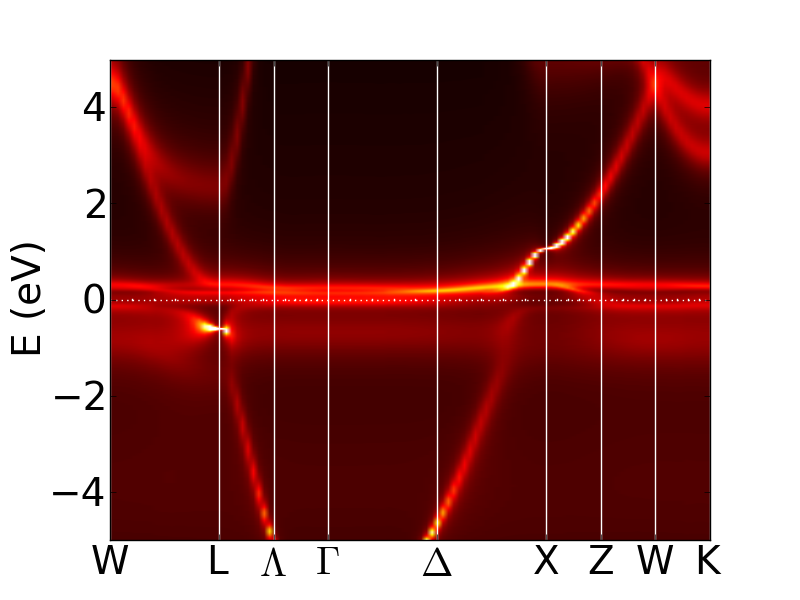
\includegraphics[scale=0.43]{FCC_FeBandStructure}
  \end{figure}

  \cleardoublepage

      \subsubsection{Optics including conductivity}

  \begin{enumerate}

    \item Preparation: make a new folder in \emph{FCC\_Fe},

  \textbf{mkdir -p FCC\_Fe/optics/FCC\_Fe}

    \item Copy all the required files from DMFT calculations to the current directory,

  \textbf{dmft\_copy.py ../../ -a}

    \item Prepare \emph{FCC\_Fe.inop} file. Refer to WIEN2k userguide for example of \emph{.inop} file. It should 
contain the following information.   

{\color{cyan}

99999 1      : NKMAX, NKFIRST

-5.0 5.0     : EMIN, EMAX, NBvalMAX

3            : number of choices (columns in *symmat)

1            : Re xx

2            : Re yy

3            : Re zz

ON           : ON/OFF writes MME to unit 4

}

    \item Prepare \emph{dmftopt.in} file. Make sure ``\# dwindow'' value is large enough to get better results. Below 
shows the contents of this file.

{\color{cyan}

    0          \# updn: [0|up|dn] -- 0 for non-magnetic calculation

    Fe         \# case

    0.01       \# gamma  -- broadening of all bands / we recommend to keep nonzero value

    0.0        \# gammac -- broadening of the correlated bands (in addition to the self-energy)

    15         \# ommax  -- maximum frequency for the optics calculation

    1e-2       \# delta  -- minimum separation of frequency for logarithmic mesh in frequency

    8          \# Nd     -- number of points in each linear mesh, a subset of logarithmic mesh

    T          \# Qsym: [F|T]. Do we need to symmetrize? (over all irreducible only or over all.)

    F          \# InterbandOnly [F|T] (F -- all, T--interband)

    20         \# dwindow -- Not all bands are used in computation of optics, but only those from [-omeg-dwindow, 
omega+dwindow].

    3          \# Ndirection -- How many optics type do you want to compute: xx, yy, zz,...

    1.0 0.0 0.0    \# alphaV(1,:)

    0.0 0.0 0.0    \# alphaV(2,:)

    0.0 0.0 0.0    \# alphaV(3,:)

    0.0 0.0 0.0    \# alphaV(1,:)

    0.0 1.0 0.0    \# alphaV(2,:)

    0.0 0.0 0.0    \# alphaV(3,:)

    0.0 0.0 0.0    \# alphaV(1,:)

    0.0 0.0 0.0    \# alphaV(2,:)

    0.0 0.0 1.0    \# alphaV(3,:)
}

    \item Replace the imaginary self-energy by self-energy in real frequency. 

  \textbf{cp /FCC\_Fe/mem/Sig\_real/Sig.out sig.inp}

    \item Edit \emph{FCC\_Fe.indmfl} file. 

  On the second line of \emph{FCC\_Fe.indmfl} file, Change the ``\emph{matsubara}'' value from \textbf{1} to 
\textbf{0} in order to switch from imaginary axis to real axis.

    \item Run \textbf{x kgen} and specify number of k-points in whole cell, \textbf{8000}

    \item Run the following commands to execute DMFT calculations in the \emph{/optics/FCC\_Fe/} directory.

  \textbf{x lapw0}

  \textbf{x lapw1}

  \textbf{x optic}

  \textbf{cp FCC\_Fe.mommat2 FCC\_Fe.mommat}

  \textbf{ssplit.py -i sig.inp}

  \textbf{x\_dmft.py dmftu}

  \textbf{dmftopt}

    \item Plot the results stored in files, \emph{optics.dat} and \emph{optdos.dat}. See Figures 
\ref{Optics properties of FCC Fe}, \ref{Density of States based on optics calculations and comparison with Total DOS 
for FCC Fe}.

  \begin{figure}[ht]
    \centering
    \caption{Optical conductivity of FCC Fe}
    \label{Optics properties of FCC Fe}
    \vspace{2ex}
    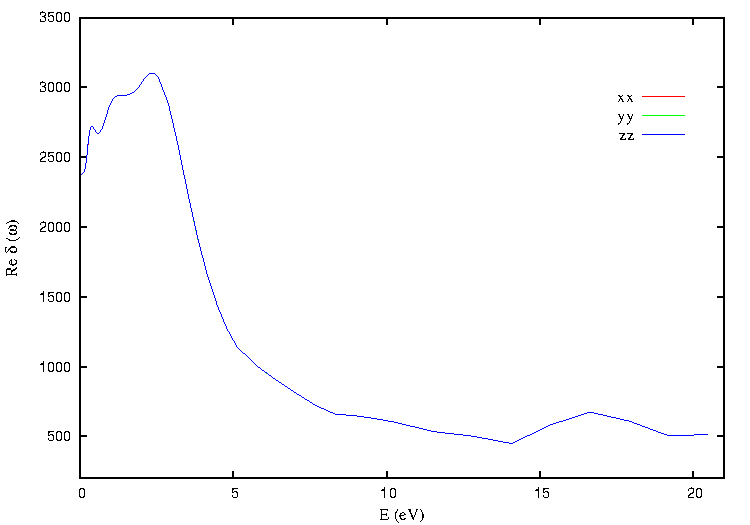
\includegraphics[scale=1.3]{gnuplotOptics}
  \end{figure}

  \begin{figure}[ht]
    \centering
    \captionsetup{justification=centering}
    \caption{Density of States based on optics calculations and comparison with Total DOS for FCC Fe}
    \label{Density of States based on optics calculations and comparison with Total DOS for FCC Fe}
    \vspace{2ex}
    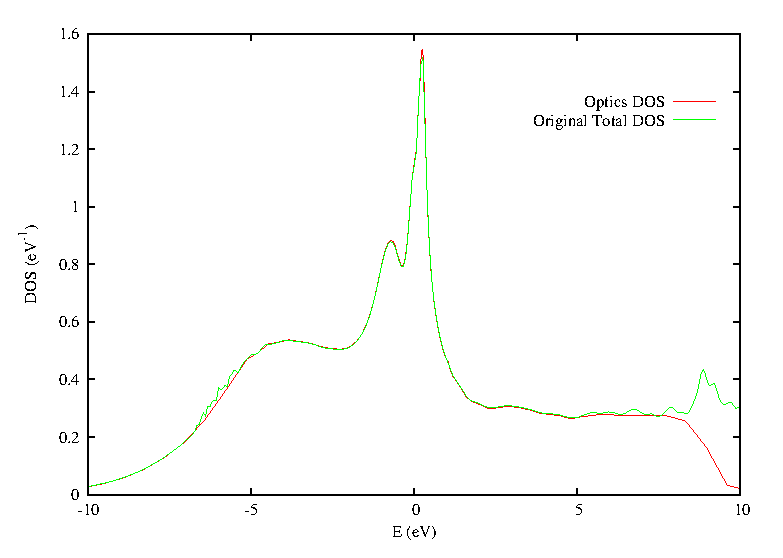
\includegraphics[scale=1.3]{gnuplotOptDOS}
  \end{figure}

  \end{enumerate}

  \cleardoublepage

      \subsubsection{Fermi Surface}





  \clearpage
  \addcontentsline{toc}{part}{References}
  \bibliographystyle{plainnat} 			% set bibliography style
  \bibliography{DFT+DMFT_usersguide_v3} 		% include bibliography files

  \clearpage
  \appendixtitleon
  \appendixtitletocon
  \begin{appendices}
       
%     \section{Params.dat}
% 
%   \begin{figure}[ht]
%     \centering
%     \caption{Parameters file}
%     \label{Parameters file}
%     \vspace{2ex}
%     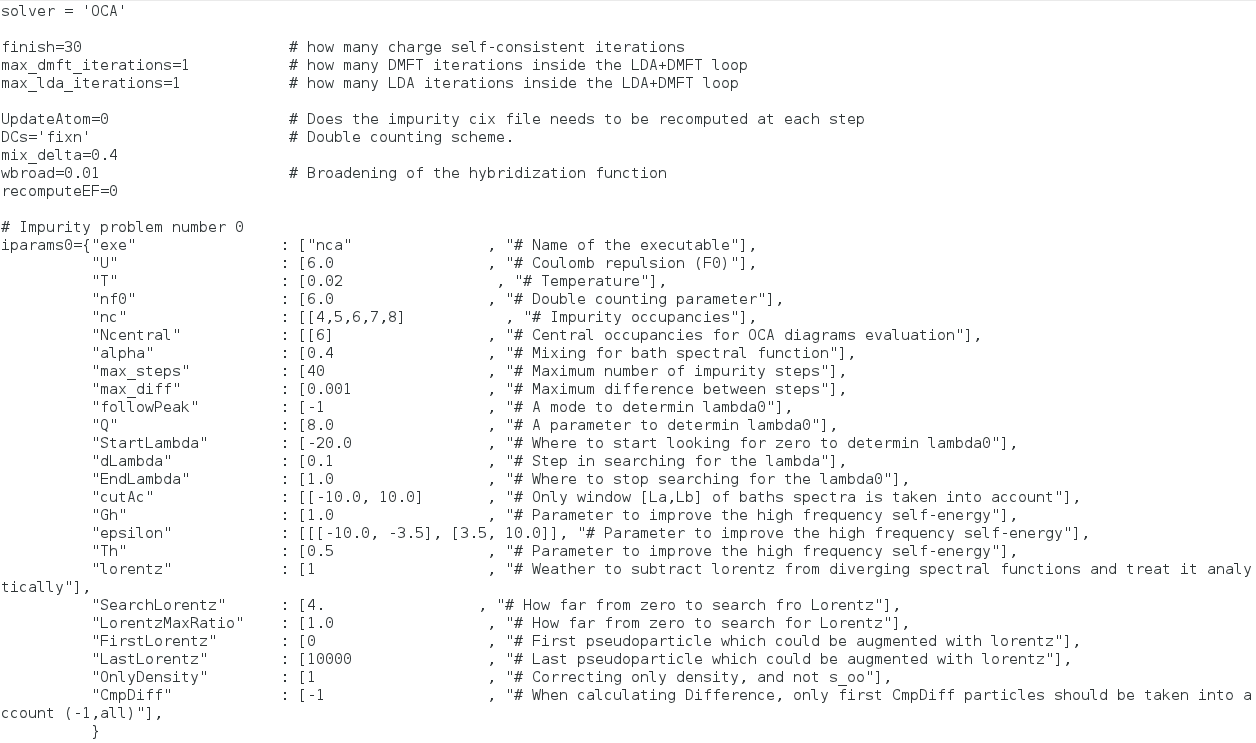
\includegraphics[scale = 0.36]{paramsdat}
%   \end{figure}
%   \clearpage

%     \section{Files generated after each step}
% 
%   \begin{figure}[ht]
%    \centering
%    \includegraphics[scale=0.42]{FilesStep1}
%    %\caption{Files generated Step 1}
%   \end{figure}
% 
%   \begin{figure}
%    \centering
%    \includegraphics[scale=0.42]{FilesStep2}
%    %\caption{Files generated Step 2}
%   \end{figure}
% 
%   \begin{figure}
%    \centering
%    \includegraphics[scale=0.42]{FilesStep3}
%    %\caption{Files generated Step 3}
%   \end{figure}
% 
%   \begin{figure}
%    \centering
%    \includegraphics[scale=0.42]{FilesStep4}
%    %\caption{Files generated Step 4}
%   \end{figure}
% 
%   \begin{figure}
%    \centering
%    \includegraphics[scale=0.42]{FilesStep5}
%    %\caption{Files generated Step 5}
%   \end{figure}
%   \cleardoublepage


  \clearpage % add page after contents

  \end{appendices}

\end{document}

